%%%%%%%%%%%%%%%%%%%%%%%%%%%%%%%%%%%%%%%%%%%%%%%%%%%%%%%%%%%%%%%%%%%%%%
%%%%% Configuration %%%%%%%%%%%%%%%%%%%%%%%%%%%%%%%%%%%%%%%%%%%%%%%%%%
%%%%%%%%%%%%%%%%%%%%%%%%%%%%%%%%%%%%%%%%%%%%%%%%%%%%%%%%%%%%%%%%%%%%%%

\documentclass[
	a4paper,	% feuille A4
	twoside,	% impression Recto simple
	11 pt		% taille de police
]{report}		% type de document


%%%%%%%%%% Extensions %%%%%%%%%%
\usepackage[utf8]{inputenc}		% encodage des caractères
\usepackage[T1]{fontenc}		% nouvelle norme de codage
\usepackage[francais]{babel}	% langue française
\usepackage{lscape}				% format paysage
\usepackage{multicol}			% multi-colonnes
\usepackage{graphicx}			% images
\usepackage{float}				% insertion d'image avec l'option "H"
\usepackage{textcomp}			% signe €


%%%%%%%%%% Numérotation des paragraphes %%%%%%%%%%
\setcounter{secnumdepth}{3}		% corps
\setcounter{tocdepth}{3}		% table des matières


%%%%%%%%%% Marges %%%%%%%%%%
\usepackage[
	tmargin = 2.7 cm,	% haut
	bmargin = 5 cm,		% bas
	lmargin = 2.5 cm,	% gauche
	rmargin = 2.5 cm	% droite
]{geometry}


%%%%%%%%%% Inter-ligne %%%%%%%%%%
\usepackage{setspace}
\onehalfspacing			% 1.5


%%%%%%%%%% Code source %%%%%%%%%%
\usepackage{listings}
\lstset{
	showstringspaces = false,	% masquer les espaces
	tabsize = 4,				% nombre d'espace par tabulation
	basicstyle=\ttfamily,		% caractères de même taille
	xleftmargin = 30 pt,		% marge à gauche
	xrightmargin = 0 pt,		% marge à droite
	aboveskip = -1 pt,			% espace au dessus de la zone
	belowskip = -1 pt			% espace en dessous de la zone
}


%%%%%%%%%% Informations %%%%%%%%%%
\title{Communication entre smartphone et ordinateur}
\author{\href{mailto:matsuhar@gmail.com}{Iori MATSUHARA}, \href{mailto:pinguet62@gmail.com}{Julien PINGUET}}
\date{Octobre 2012-Mars 2013}


%%%%%%%%%% Liens %%%%%%%%%%
\usepackage{hyperref}
\hypersetup{
	backref = true,
	pagebackref = true,	% dans bibliographie
	pdfborder = {0 0 0}	% retirer le cadre
}


%%%%%%%%%% Glossaire %%%%%%%%%%
\usepackage{glossaries}
\makeglossaries



\storeglosentry{vbox}{
	name = {
		VirtualBox
	},
	description = {
		C'est un logiciel de virtualisation, compatible multiplateforme (Windows, Unix, Mac OS X, \dot), développé par Oracle.
	}
}



\storeglosentry{virtualisation}{
	name = {
		Virtualisation
	},
	description = {
		Consiste à émuler un ou plusieurs systèmes d'exploitation, au sein même d'un autre système d'exploitation.
	}
}



\storeglosentry{Python}{
	name = {
		Python
	},
	description = {
		Langage de programmation multi-paradigme, à typage dynamique fort , et orienté objet.
	}
}


%%%%%%%%%% Notes de bas de page %%%%%%%%%%
\usepackage[bottom]{footmisc}	% Collé au bas de page


%%%%%%%%%% En-tête et Pied de page %%%%%%%%%%
\usepackage{fancyhdr}
\makeatletter % début d'utilisation des variables @



%%%%%%%%%%%%%%%%%%%%%%%%%%%%%%%%%%%%%%%%%%%%%%%%%%%%%%%%%%%%%%%%%%%%%%%%%%%%%%%%%%%%%%%%%%%%%%%%%%%%
%%%%% Page vides %%%%%%%%%%%%%%%%%%%%%%%%%%%%%%%%%%%%%%%%%%%%%%%%%%%%%%%%%%%%%%%%%%%%%%%%%%%%%%%%%%%
%%%%%%%%%%%%%%%%%%%%%%%%%%%%%%%%%%%%%%%%%%%%%%%%%%%%%%%%%%%%%%%%%%%%%%%%%%%%%%%%%%%%%%%%%%%%%%%%%%%%

\fancypagestyle{empty}{
	% Effacer les valeurs par défaut
	\fancyhf{}
	
	% Remplissage
	\lhead	[]								% haut	gauche	pair
			{}								% haut	gauche	impair
	\chead	[]								% haut	centre	pair
			{}								% haut	centre	impair
	\rhead	[]								% haut	droite	pair
			{}								% haut	droite	impair
	\lfoot	[]								% bas	gauche	pair
			{}								% bas	gauche	impair
	\cfoot	[]								% bas	centre	pair
			{}								% bas	centre	impair
	\rfoot	[]								% bas	droite	pair
			{}								% bas	droite	impair
	
	% Epaisseur de la ligne séparatrice
	\renewcommand{\headrulewidth}{0 pt}		% en-tête (défaut : 0.4pt)
	\renewcommand{\footrulewidth}{0 pt}		% pied de page (défaut : 0pt)
	
	% Distance du corps
	\headsep = 25 pt						% en-tête (défaut : 25pt)
	\footskip = 75 pt						% pied de page (défaut : 30pt)
}



%%%%%%%%%%%%%%%%%%%%%%%%%%%%%%%%%%%%%%%%%%%%%%%%%%%%%%%%%%%%%%%%%%%%%%%%%%%%%%%%%%%%%%%%%%%%%%%%%%%%
%%%%% Page des chapitre (défaut) %%%%%%%%%%%%%%%%%%%%%%%%%%%%%%%%%%%%%%%%%%%%%%%%%%%%%%%%%%%%%%%%%%
%%%%%%%%%%%%%%%%%%%%%%%%%%%%%%%%%%%%%%%%%%%%%%%%%%%%%%%%%%%%%%%%%%%%%%%%%%%%%%%%%%%%%%%%%%%%%%%%%%%%

\fancypagestyle{plain}{
	% Effacer les valeurs par défaut
	\fancyhf{}
	
	% Remplissage
	\lhead	[\large \bf \fbox{\thepage}]	% haut	gauche	pair	:	numéro de page
			{}								% haut	gauche	impair
	\chead	[]								% haut	centre	pair
			{}								% haut	centre	impair
	\rhead	[]								% haut	droite	pair
			{\large \bf \fbox{\thepage}}	% haut	droite	impair	:	numéro de page
	\lfoot	[\@title]						% bas	gauche	pair	:	titre du rapport
			{\@author}						% bas	gauche	impair	:	auteur du rapport
	\cfoot	[]								% bas	centre	pair
			{}								% bas	centre	impair
	\rfoot	[\@author]						% bas	droite	pair	:	auteur du rapport
			{\@title}						% bas	droite	impair	:	titre du rapport
	
	% Epaisseur de la ligne séparatrice
	\renewcommand{\headrulewidth}{0 pt}		% en-tête (défaut : 0.4pt)
	\renewcommand{\footrulewidth}{0.4 pt}	% pied de page (défaut : 0pt)
	
	% Distance du corps
	\headsep = 25 pt						% en-tête (défaut : 25pt)
	\footskip = 75 pt						% pied de page (défaut : 30pt)
}



%%%%%%%%%%%%%%%%%%%%%%%%%%%%%%%%%%%%%%%%%%%%%%%%%%%%%%%%%%%%%%%%%%%%%%%%%%%%%%%%%%%%%%%%%%%%%%%%%%%%
%%%%% Corps du rapport (hors page de chapitre) %%%%%%%%%%%%%%%%%%%%%%%%%%%%%%%%%%%%%%%%%%%%%%%%%%%%%
%%%%%%%%%%%%%%%%%%%%%%%%%%%%%%%%%%%%%%%%%%%%%%%%%%%%%%%%%%%%%%%%%%%%%%%%%%%%%%%%%%%%%%%%%%%%%%%%%%%%

\fancypagestyle{corps}{
	% Effacer les valeurs par défaut
	\fancyhf{}
	
	% Remplissage
	\lhead	[\large \bf \thepage]				% haut	gauche	pair	:	numéro de page
			{\bf \nouppercase \rightmark}		% haut	gauche	impair	:	nom de la section
	\chead	[]									% haut	centre	pair
			{}									% haut	centre	impair
	\rhead	[\large \bf \nouppercase \leftmark]	% haut	droite	pair	:	nom du chapitre
			{\large \bf \thepage}				% haut	droite	impair	:	numéro de page
	\lfoot	[\@title]							% bas	gauche	pair	:	titre du rapport
			{\@author}							% bas	gauche	impair	:	auteur du rapport
	\cfoot	[]									% bas	centre	pair
			{}									% bas	centre	impair
	\rfoot	[\@author]							% bas	droite	pair	:	auteur du rapport
			{\@title}							% bas	droite	impair	:	titre du rapport
	
	% Epaisseur de la ligne séparatrice
	\renewcommand{\headrulewidth}{0.4 pt}		% en-tête (défaut : 0.4pt)
	\renewcommand{\footrulewidth}{0.4 pt}		% pied de page (défaut : 0pt)
	
	% Distance du corps
	\headsep = 25 pt							% en-tête (défaut : 25pt)
	\footskip = 75 pt							% pied de page (défaut : 30pt)
}



%%%%%%%%%%%%%%%%%%%%%%%%%%%%%%%%%%%%%%%%%%%%%%%%%%%%%%%%%%%%%%%%%%%%%%%%%%%%%%%%%%%%%%%%%%%%%%%%%%%%
%%%%% Annexes (hors page de chapitre) %%%%%%%%%%%%%%%%%%%%%%%%%%%%%%%%%%%%%%%%%%%%%%%%%%%%%%%%%%%%%%
%%%%%%%%%%%%%%%%%%%%%%%%%%%%%%%%%%%%%%%%%%%%%%%%%%%%%%%%%%%%%%%%%%%%%%%%%%%%%%%%%%%%%%%%%%%%%%%%%%%%

\fancypagestyle{annexe}{
	% Effacer les valeurs par défaut
	\fancyhf{}
	
	% Remplissage
	\lhead	[\large \bf \thepage]			% haut	gauche	pair	:	numéro de page
			{\bf \nouppercase \rightmark}	% haut	gauche	impair	:	nom de la section
	\chead	[]								% haut	centre	pair
			{}								% haut	centre	impair
	\rhead	[\large \bf Annexes]			% haut	droite	pair	:	"Annexes"
			{\large \bf \thepage}			% haut	droite	impair	:	numéro de page
	\lfoot	[\@title]						% bas	gauche	pair	:	titre du rapport
			{\@author}						% bas	gauche	impair	:	auteur du rapport
	\cfoot	[]								% bas	centre	pair
			{}								% bas	centre	impair
	\rfoot	[\@author]						% bas	droite	pair	:	auteur du rapport
			{\@title}						% bas	droite	impair	:	titre du rapport
	
	% Epaisseur de la ligne séparatrice
	\renewcommand{\headrulewidth}{0.4 pt}	% en-tête (défaut : 0.4pt)
	\renewcommand{\footrulewidth}{0.4 pt}	% pied de page (défaut : 0pt)
	
	% Distance du corps
	\headsep = 25 pt						% en-tête (défaut : 25pt)
	\footskip = 75 pt						% pied de page (défaut : 30pt)
}


\makeatother % fin d'utilisation des variables @
% Pas d'en-tête dans la table des matières
\makeatletter
\renewcommand{\tableofcontents}{
	\chapter*{\contentsname}
	\thispagestyle{empty}
	\@starttoc{toc}}
\makeatother


%%%%%%%%%% En-tête de chapitre %%%%%%%%%%
% Numérotation des chapitres en chiffres romains
\renewcommand{\thechapter}{\Roman{chapter}}
% Format des titres de chapitre
\makeatletter							% début d'utilisation des variables @
\def\@makechapterhead#1{
	\vspace*{50\p@} {					% espace vertical incompressible
		\parindent \z@					% indentation
		\Huge							% grande taille
		\bfseries						% texte gras
		% Si le chapitre porte un numéro
		\ifnum \m@ne < \c@secnumdepth	% secnumdepth : profondeur dans la table des matières
			\thechapter					% numéro de chapitre
			\quad						% espace horizontal moyen
		\fi
		#1								% argument : nom de chapitre
		\par
		\nobreak						% empécher le saut de page/ligne
	}
	\vskip 40\p@						% espace vertical 
}
\makeatother							% fin d'utilisation des variables @



%%%%%%%%%%%%%%%%%%%%%%%%%%%%%%%%%%%%%%%%%%%%%%%%%%%%%%%%%%%%%%%%%%%%%%
%%%%% Contenu %%%%%%%%%%%%%%%%%%%%%%%%%%%%%%%%%%%%%%%%%%%%%%%%%%%%%%%%
%%%%%%%%%%%%%%%%%%%%%%%%%%%%%%%%%%%%%%%%%%%%%%%%%%%%%%%%%%%%%%%%%%%%%%

\begin{document}

\sloppy	% ajuster correctement le texte
\renewcommand{\chaptermark}[1]{\markboth{\thechapter.\ #1}{}}	% titre chapitre
\renewcommand{\sectionmark}[1]{\markright{\thesection.\ #1}}	% titre section
\pagestyle{empty}

%%%%%%%%%% Page de garde %%%%%%%%%%
\thispagestyle{empty}

\makeatletter % début d'utilisation des variables @



\begin{multicols}{2}
	\begin{flushleft}
	
		%%%%%%%%%%%%%%%%%%%%%%%%%%%%%%%%%%%%%%%%%%%%%%%%%%%%%%%%%%%%%%%%%%%%%%
		%%%%% Haut-Gauche %%%%%%%%%%%%%%%%%%%%%%%%%%%%%%%%%%%%%%%%%%%%%%%%%%%%
		%%%%%%%%%%%%%%%%%%%%%%%%%%%%%%%%%%%%%%%%%%%%%%%%%%%%%%%%%%%%%%%%%%%%%%
	
		% Logo école
		
\includegraphics[scale=0.09]{img/ISIMA_logo.png}					\\
		
		% Nom école
		\textbf{I}nstitut \textbf{S}upérieur								\\
		d'\textbf{I}nformatique, de											\\
		\textbf{M}odélisation et de											\\
		leurs \textbf{A}pplications	
		
		\vspace*{0.5cm}
		
		% Adresse école
		BP 10125															\\
		63173 Aubière Cedex
		
		%%%%%%%%%%%%%%%%%%%%%%%%%%%%%%%%%%%%%%%%%%%%%%%%%%%%%%%%%%%%%%%%%%%%%%
		
	\end{flushleft}
\columnbreak
	\begin{flushright}
	
		%%%%%%%%%%%%%%%%%%%%%%%%%%%%%%%%%%%%%%%%%%%%%%%%%%%%%%%%%%%%%%%%%%%%%%
		%%%%% Haut-Droite %%%%%%%%%%%%%%%%%%%%%%%%%%%%%%%%%%%%%%%%%%%%%%%%%%%%
		%%%%%%%%%%%%%%%%%%%%%%%%%%%%%%%%%%%%%%%%%%%%%%%%%%%%%%%%%%%%%%%%%%%%%%
		
		%%%%%%%%%%%%%%%%%%%%%%%%%%%%%%%%%%%%%%%%%%%%%%%%%%%%%%%%%%%%%%%%%%%%%%
		
	\end{flushright}
\end{multicols}

\vspace*{\fill}

\begin{center}

	%%%%%%%%%%%%%%%%%%%%%%%%%%%%%%%%%%%%%%%%%%%%%%%%%%%%%%%%%%%%%%%%%%%%%%
	%%%%% Centre %%%%%%%%%%%%%%%%%%%%%%%%%%%%%%%%%%%%%%%%%%%%%%%%%%%%%%%%%
	%%%%%%%%%%%%%%%%%%%%%%%%%%%%%%%%%%%%%%%%%%%%%%%%%%%%%%%%%%%%%%%%%%%%%%

	% Informations
	\Large
	Rapport d'ingénieur													\\
	Projet de 3\up{ème} année											\\
	\textit{Filière :} Génie Logiciel et Systèmes Informatiques			\\
	\textit{Filière :} Réseaux et Télécommunications
	
	\rule{16cm}{2pt}													\\
	\vspace*{0.35cm}
	
	% Titre du projet
	\huge
	\textbf{\@title}													\\

	\rule{16cm}{2pt}
	
	%%%%%%%%%%%%%%%%%%%%%%%%%%%%%%%%%%%%%%%%%%%%%%%%%%%%%%%%%%%%%%%%%%%%%%

\end{center}
	
\vspace*{\fill}

\begin{multicols}{2}
	\vspace*{\fill}
	% Bas-Gauche : Auteurs + Encadreur
	\begin{flushleft}
	
		%%%%%%%%%%%%%%%%%%%%%%%%%%%%%%%%%%%%%%%%%%%%%%%%%%%%%%%%%%%%%%%%%%%%%%
		%%%%% Bas-Gauche %%%%%%%%%%%%%%%%%%%%%%%%%%%%%%%%%%%%%%%%%%%%%%%%%%%%%
		%%%%%%%%%%%%%%%%%%%%%%%%%%%%%%%%%%%%%%%%%%%%%%%%%%%%%%%%%%%%%%%%%%%%%%
	
		% Auteur & Encadrants
		\textit{Présenté par :} \@author									\\
		\mbox{\textit{Sous la direction de :} Loïc YON}
		
		%%%%%%%%%%%%%%%%%%%%%%%%%%%%%%%%%%%%%%%%%%%%%%%%%%%%%%%%%%%%%%%%%%%%%%
		
	\end{flushleft}
\columnbreak
	\vspace*{\fill}
	
	\begin{flushright}
	
		%%%%%%%%%%%%%%%%%%%%%%%%%%%%%%%%%%%%%%%%%%%%%%%%%%%%%%%%%%%%%%%%%%%%%%
		%%%%% Bas-Droite %%%%%%%%%%%%%%%%%%%%%%%%%%%%%%%%%%%%%%%%%%%%%%%%%%%%%
		%%%%%%%%%%%%%%%%%%%%%%%%%%%%%%%%%%%%%%%%%%%%%%%%%%%%%%%%%%%%%%%%%%%%%%
		
		% Date
		\@date
		
		%%%%%%%%%%%%%%%%%%%%%%%%%%%%%%%%%%%%%%%%%%%%%%%%%%%%%%%%%%%%%%%%%%%%%%
		
	\end{flushright}
\end{multicols}



\makeatother % fin d'utilisation des variables @


%%%%%%%%%% Remerciements %%%%%%%%%%
\cleardoublepage



\chapter*{Remerciements}

\thispagestyle{empty}



Avant toute chose, nous tenons à remercier les personnes qui ont acceptés de nous encadrer pour effectuer ce projet.
\\


Nous remercions tout d'abord Loïc YON, docteur ingénieur en informatique et enseignant à l'ISIMA, qui nous a encadré durant ce projet.

Nous remercions aussi Patrice LAURENÇOT, chercheur et enseignant à l'ISIMA, pour avoir accepté notre proposition de projet.
\\


%%%%%%%%%% Glossaire %%%%%%%%%%
%\printglossary

%%%%%%%%%% Résumé %%%%%%%%%%
\newpage



\chapter*{Résumé}

\thispagestyle{empty}



Notre projet de dernière année à l'ISIMA avait pour but de créer une solution d'envoi et de réception de SMS à partir d'un ordinateur, en utilisant le forfait téléphonique du smartphone.
\\


Tout d'abord nous avons étudié le protocole XMPP et de GTalk qui serviront de moyen de communication entre l'ordinateur et le smartphone.
Cette analyse a permis de découvrir certains inconvénients et de comparer les différentes solutions possible.
Nous avons pu nous tourner vers la solution optimale et pratique pour l'utilisateur.

La seconde phase a consisté à développer la solution.
Nous avons développé le site web en utilisant le framework "Play", ainsi que les applications mobiles sous Androïd et iOS.

Une fois la solution finale obtenue il nous restait plus qu'à la tester et étudier les différentes améliorations possibles pour proposer une solution optimale à l'utilisateur.
Nous avons aussi ajouté quelques fonctionnalités pour compléter notre solution.
\\



\textbf{Mots clé : }
SMS, XMPP, Androïd, iOS, Play Framework


%%%%%%%%%% Abstract %%%%%%%%%%
\cleardoublepage



\chapter*{Abstract}

\thispagestyle{empty}



During my ISIMA second year studies, my work placement's aim was to build a virtualization solution in order to run scientific tools only available under Linux.
\\



I have first built and configured a full Linux virtual machine, on which my first solution will be based.
Its full development environment will compile scientific tools.

In analyzing the different techniques that could exist and be usable, I could turn towards the solutions I will use.
I have to think about the most practical solution for users but also for its development in the firm.

It will be necessary to improve the different remaining problems once the programs are developed and tests are performed. 
Then, a new minimal virtual machine that will offer better performance could be built.
\\



\textbf{Keywords : }
Virtualisation, VirtualBox, VBoxManage, Scientific tool, Python, wxPython

%%%%%%%%%% Table des matières %%%%%%%%%%
\cleardoublepage
\tableofcontents

%%%%%%%%%% Table des figures %%%%%%%%%%
\cleardoublepage
\listoffigures
\thispagestyle{empty}

%%%%%%%%%% Corps du rapport %%%%%%%%%%
\cleardoublepage
\pagestyle{corps}
\pagenumbering{arabic} % pagination en chiffres arabes

%%%%%%%%%% Introduction %%%%%%%%%%
\newpage



\chapter*{Introduction}
\addcontentsline{toc}{chapter}{Introduction}

%%%%%%%%%%%%%%%%%%%%%%%%%%%%%%%%%%%%%%%%%%%%%%%%%%%%%%%%%%%%%%%%%%%%%%%%%%%%%%%%%%%%%%%%%%%%%%%%%%%%
%%%%%%%%%% Context %%%%%%%%%%%%%%%%%%%%%%%%%%%%%%%%%%%%%%%%%%%%%%%%%%%%%%%%%%%%%%%%%%%%%%%%%%%%%%%%%
%%%%%%%%%%%%%%%%%%%%%%%%%%%%%%%%%%%%%%%%%%%%%%%%%%%%%%%%%%%%%%%%%%%%%%%%%%%%%%%%%%%%%%%%%%%%%%%%%%%%

L'envoi de SMS depuis un ordinateur est très souvent fastidieux car il n'existe quasiment aucune solution simple, gratuite et pratique.
En effet, dans la majorité des solutions existantes sont soit payantes, soit limitent leurs services à quelques envois.

Les opérateurs de téléphonie mobile proposent tous des forfait avec un envoi illimité de SMS, mais ne proposent aucune solution d'envoi à partir d'un ordinateur.
\\



%%%%%%%%%%%%%%%%%%%%%%%%%%%%%%%%%%%%%%%%%%%%%%%%%%%%%%%%%%%%%%%%%%%%%%%%%%%%%%%%%%%%%%%%%%%%%%%%%%%%
%%%%%%%%%% Problème %%%%%%%%%%%%%%%%%%%%%%%%%%%%%%%%%%%%%%%%%%%%%%%%%%%%%%%%%%%%%%%%%%%%%%%%%%%%%%%%
%%%%%%%%%%%%%%%%%%%%%%%%%%%%%%%%%%%%%%%%%%%%%%%%%%%%%%%%%%%%%%%%%%%%%%%%%%%%%%%%%%%%%%%%%%%%%%%%%%%%

Comment pourrait-on utiliser notre forfait téléphonique pour envoyer des SMS depuis l'ordinateur ?
Quelle serait la solution la plus pratique pour l'utilisateur ?
\\



%%%%%%%%%%%%%%%%%%%%%%%%%%%%%%%%%%%%%%%%%%%%%%%%%%%%%%%%%%%%%%%%%%%%%%%%%%%%%%%%%%%%%%%%%%%%%%%%%%%%
%%%%%%%%%% Objectif %%%%%%%%%%%%%%%%%%%%%%%%%%%%%%%%%%%%%%%%%%%%%%%%%%%%%%%%%%%%%%%%%%%%%%%%%%%%%%%%
%%%%%%%%%%%%%%%%%%%%%%%%%%%%%%%%%%%%%%%%%%%%%%%%%%%%%%%%%%%%%%%%%%%%%%%%%%%%%%%%%%%%%%%%%%%%%%%%%%%%

L'objet de cette étude sera d'étudier et de développer une solution d'envoi de SMS depuis un ordinateur, simple pour l'utilisateur et utilisable par tous.
Cette solution se basera sur la communication entre le smartphone et l'ordinateur, qui s'échangeront les informations du SMS.
\\



%%%%%%%%%%%%%%%%%%%%%%%%%%%%%%%%%%%%%%%%%%%%%%%%%%%%%%%%%%%%%%%%%%%%%%%%%%%%%%%%%%%%%%%%%%%%%%%%%%%%
%%%%%%%%%% Démarche et plan %%%%%%%%%%%%%%%%%%%%%%%%%%%%%%%%%%%%%%%%%%%%%%%%%%%%%%%%%%%%%%%%%%%%%%%%
%%%%%%%%%%%%%%%%%%%%%%%%%%%%%%%%%%%%%%%%%%%%%%%%%%%%%%%%%%%%%%%%%%%%%%%%%%%%%%%%%%%%%%%%%%%%%%%%%%%%

%%%%%%%%%% Démarche %%%%%%%%%%%%%%%%%%%%%%%%%%%%%%%%%%%%%%%%%%%%%%%%%%%%%%%%%%%%%%%%%%%%%%%%%%%%%%%%

L'étude des différentes solutions possibles permettra de les tester et de comparer leurs avantages et défauts pour mieux nous amener vers la solution pratique et optimale.
Une fois la solution choisie elle sera développée pour permettre son utilisation.
Enfin il ne restera plus qu'à l'optimiser et lui apporter de nouvelles fonctionnalités.

%%%%%%%%%% Plan %%%%%%%%%%%%%%%%%%%%%%%%%%%%%%%%%%%%%%%%%%%%%%%%%%%%%%%%%%%%%%%%%%%%%%%%%%%%%%%%%%%%

Tous d'abord nous présenterons la démarche suivie pour nous orienter vers la solution envisagée.
Dans un deuxième temps nous présenterons les outils utilisés et les techniques mises en œuvre pour développer le projet.
Pour terminer nous présenterons la solution finale obtenue et discuterons des améliorations possibles.
\\


%%%%%%%%%% Chapitre 1 %%%%%%%%%%
\cleardoublepage



\chapter{Introduction de l'étude}
\label{Introduction de l'étude}

%%%%%%%%%%%%%%%%%%%%%%%%%%%%%%%%%%%%%%%%%%%%%%%%%%%%%%%%%%%%%%%%%%%%%%%%%%%%%%%%%%%%%%%%%%%%%%%%%%%%
%%%%%%%%%%%%%%%%%%%%%%%%%%%%%%%%%%%%%%%%%%%%%%%%%%%%%%%%%%%%%%%%%%%%%%%%%%%%%%%%%%%%%%%%%%%%%%%%%%%%
%%%%%%%%%%%%%%%%%%%%%%%%%%%%%%%%%%%%%%%%%%%%%%%%%%%%%%%%%%%%%%%%%%%%%%%%%%%%%%%%%%%%%%%%%%%%%%%%%%%%
%%%%%%%%%%%%%%%%%%%%%%%%%%%%%%%%%%%%%%%%%%%%%%%%%%%%%%%%%%%%%%%%%%%%%%%%%%%%%%%%%%%%%%%%%%%%%%%%%%%%
%%%%%%%%%%%%%%%%%%%%%%%%%%%%%%%%%%%%%%%%%%%%%%%%%%%%%%%%%%%%%%%%%%%%%%%%%%%%%%%%%%%%%%%%%%%%%%%%%%%%

\section{Besoin de l'utilisateur}

L'envoi de SMS depuis son ordinateur possède plusieurs avantages par rapport à l'envoi depuis un smartphone.
\\


Il est beaucoup plus aisé d'écrire un texte depuis un clavier d'ordinateur, plutôt que sur un écran tactile ou un clavier à très petites touches.
Cela peut aussi aider les personnes ayant des difficultés avec les smartphones, comme par exemple les personnes malvoyantes.
\\


Tout le monde n'a pas accès instantanément à son smartphone lorsque l'on utilise un ordinateur.
Celui-ci peut être dans notre poche, dans un sac, posé sur une table distante, \ldots et l'on aimerait écrire lire ou répondre à des SMS sans avoir à se déplacer tout en gardant les yeux sur l'écran et les mains sur le clavier.
\\





%%%%%%%%%%%%%%%%%%%%%%%%%%%%%%%%%%%%%%%%%%%%%%%%%%%%%%%%%%%%%%%%%%%%%%%%%%%%%%%%%%%%%%%%%%%%%%%%%%%%
%%%%%%%%%%%%%%%%%%%%%%%%%%%%%%%%%%%%%%%%%%%%%%%%%%%%%%%%%%%%%%%%%%%%%%%%%%%%%%%%%%%%%%%%%%%%%%%%%%%%
%%%%%%%%%%%%%%%%%%%%%%%%%%%%%%%%%%%%%%%%%%%%%%%%%%%%%%%%%%%%%%%%%%%%%%%%%%%%%%%%%%%%%%%%%%%%%%%%%%%%
%%%%%%%%%%%%%%%%%%%%%%%%%%%%%%%%%%%%%%%%%%%%%%%%%%%%%%%%%%%%%%%%%%%%%%%%%%%%%%%%%%%%%%%%%%%%%%%%%%%%
%%%%%%%%%%%%%%%%%%%%%%%%%%%%%%%%%%%%%%%%%%%%%%%%%%%%%%%%%%%%%%%%%%%%%%%%%%%%%%%%%%%%%%%%%%%%%%%%%%%%

\section{Solutions existantes}

Les solutions actuellement proposées aux utilisateurs sont très limitées, ce qui explique le fait que très peux d'entre-eux sont utilisées.
\\


Chez certains opérateurs de téléphonie mobile le service SMS peut couter plus de 0,10\texteuro par envoi, et les tarifs des sites indépendants affichent des prix voisins.
Des solutions gratuites existent et permettent des envois gratuits sur internet, mais ceux-ci sont limités à quelques envois ou bien demande une confirmation pour éviter les abus.

Un inconvénient remarquable parmi toutes les solutions existantes est l'absence de gestion des contacts.
En effet l'utilisateur est obligé de spécifier "à la main" le numéro de téléphone du destinataire.
Cela est fastidieux car il faut soit connaitre le numéro par cœur, soit accéder à son carnet d'adresse qui se trouve souvent sur son smartphone.

La dernière remarque que nous pouvons faire sur les solutions existantes est le fait que la réception des SMS n'est gérée.
Cela peut s'expliquer par le fait que la réception de SMS nécessite une mémorisation du message (dans le logiciel ou sur le serveur web), contrairement à l'envoi.
\\





%%%%%%%%%%%%%%%%%%%%%%%%%%%%%%%%%%%%%%%%%%%%%%%%%%%%%%%%%%%%%%%%%%%%%%%%%%%%%%%%%%%%%%%%%%%%%%%%%%%%
%%%%%%%%%%%%%%%%%%%%%%%%%%%%%%%%%%%%%%%%%%%%%%%%%%%%%%%%%%%%%%%%%%%%%%%%%%%%%%%%%%%%%%%%%%%%%%%%%%%%
%%%%%%%%%%%%%%%%%%%%%%%%%%%%%%%%%%%%%%%%%%%%%%%%%%%%%%%%%%%%%%%%%%%%%%%%%%%%%%%%%%%%%%%%%%%%%%%%%%%%
%%%%%%%%%%%%%%%%%%%%%%%%%%%%%%%%%%%%%%%%%%%%%%%%%%%%%%%%%%%%%%%%%%%%%%%%%%%%%%%%%%%%%%%%%%%%%%%%%%%%
%%%%%%%%%%%%%%%%%%%%%%%%%%%%%%%%%%%%%%%%%%%%%%%%%%%%%%%%%%%%%%%%%%%%%%%%%%%%%%%%%%%%%%%%%%%%%%%%%%%%
%%%%%%%%%%%%%%%%%%%%%%%%%%%%%%%%%%%%%%%%%%%%%%%%%%%%%%%%%%%%%%%%%%%%%%%%%%%%%%%%%%%%%%%%%%%%%%%%%%%%

\section{Solution envisagée}

Pour établir notre cahier des charges nous avons étudié les solutions existantes puis étudiés leurs principaux défauts pour produite une solution optimale pour l'utilisateur.
\\


Sachant que la quasi totalité des forfaits mobiles autorisent un nombre illimité d'envois de SMS, nous voulons donc que les utilisateurs utilisent leur propre forfait mobile pour effectuer les envois et réceptions de SMS depuis l'ordinateur, en utilisant un protocole de communication qui transférerait les données.

Nous avons décidé d'intégrer la réception des SMS dans notre solution.
Cette fonctionnalité devra se faire de manière sécurisée et confidentielle.

Enfin nous avons voulu proposer une gestion simple des contacts de l'utilisateur lui permettant de ne pas à avoir à entrer le numéro de téléphone.
De même que pour la réception des SMS, les contacts devront être sûre.
\\


Le schéma ci-dessous représente le fonctionnement général de la solution.
Les flèches vertes indiquent le cheminement du message lors de l'envoi, et les flèches bleues indiquent le cheminement du message lors de la réception.

\begin{figure}[!h]
	\center
	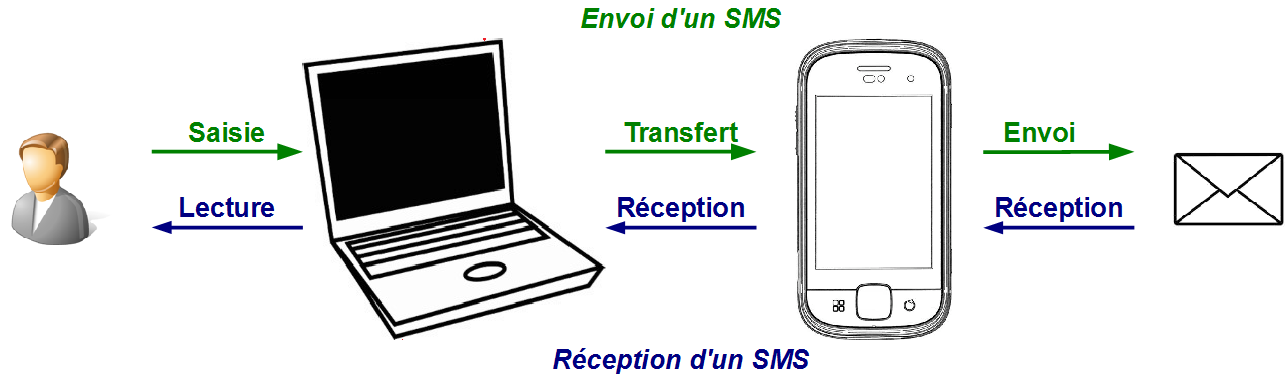
\includegraphics[width=0.9\textwidth]{img/schemaFonctionnement_general.png}
	\caption{Fonctionnement général}
	\label{schemaFonctionnement_general}
\end{figure}


%%%%%%%%%% Chapitre 2 %%%%%%%%%%
\cleardoublepage



\chapter{Recherche de la solution optimale}

La première partie de notre projet a consisté à étudier les différentes étapes du fonctionnement de notre solution : de la réception d'un SMS sur le smartphone à son affichage sur l'ordinateur, mais aussi de l'écriture d'un message sur l'ordinateur jusqu'à son envoi par le smartphone.
L'objectif de cette étude était de trouver la solution optimale que nous développeront pour ce projet.
Nous détaillerons plus précisément le choix du service proposé à l'utilisateur pour l'envoi du SMS depuis l'ordinateur.





%%%%%%%%%%%%%%%%%%%%%%%%%%%%%%%%%%%%%%%%%%%%%%%%%%%%%%%%%%%%%%%%%%%%%%%%%%%%%%%%%%%%%%%%%%%%%%%%%%%%
%%%%%%%%%%%%%%%%%%%%%%%%%%%%%%%%%%%%%%%%%%%%%%%%%%%%%%%%%%%%%%%%%%%%%%%%%%%%%%%%%%%%%%%%%%%%%%%%%%%%
%%%%%%%%%%%%%%%%%%%%%%%%%%%%%%%%%%%%%%%%%%%%%%%%%%%%%%%%%%%%%%%%%%%%%%%%%%%%%%%%%%%%%%%%%%%%%%%%%%%%
%%%%%%%%%%%%%%%%%%%%%%%%%%%%%%%%%%%%%%%%%%%%%%%%%%%%%%%%%%%%%%%%%%%%%%%%%%%%%%%%%%%%%%%%%%%%%%%%%%%%
%%%%%%%%%%%%%%%%%%%%%%%%%%%%%%%%%%%%%%%%%%%%%%%%%%%%%%%%%%%%%%%%%%%%%%%%%%%%%%%%%%%%%%%%%%%%%%%%%%%%

\section{Les application mobiles}

Il est nécessaire que l'utilisateur installe une application sur son smartphone pour réagir aux réception de SMS et aux demandes d'envoi de l'utilisateur.
\\


Lors de la réception d'un SMS, l'application va recevoir une événement puis va lire le dernier SMS reçu.
Une fois le contenu et l'expéditeur du SMS lus, l'application va envoyer le message "sur l'ordinateur" de l'utilisateur pour l'avertir de la réception.

Lors de la réception d'un message (contenu du SMS et destinataire) provenant de "l'ordinateur" de l'utilisateur, l'application va envoyer le SMS au destinataire.
Cet envoi doit bien évidemment se faire de manière automatique et transparente.

Le schéma \ref{schemaFonctionnement_applicationMobile} représente le fonctionnement global des applications mobiles qui seront utilisées dans notre projet.
\begin{figure}[!h]
	\center
	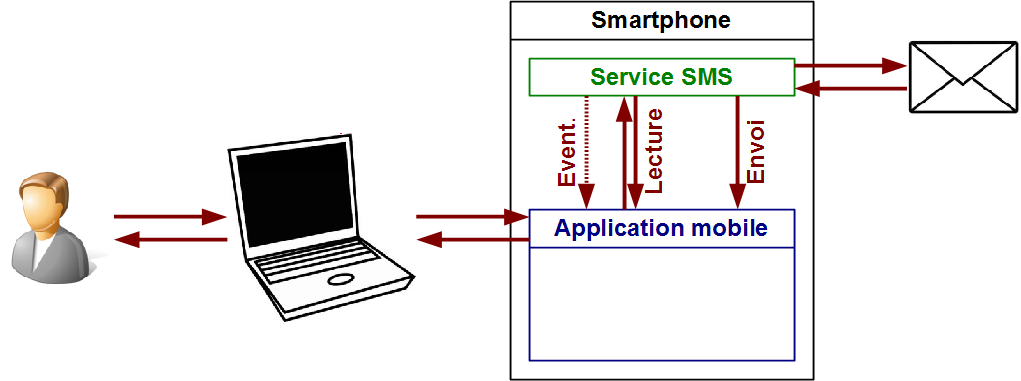
\includegraphics[width=0.9\textwidth]{img/schemaFonctionnement_applicationMobile.png}
	\caption{Applications mobiles : fonctionnement}
	\label{schemaFonctionnement_applicationMobile}
\end{figure}





%%%%%%%%%%%%%%%%%%%%%%%%%%%%%%%%%%%%%%%%%%%%%%%%%%%%%%%%%%%%%%%%%%%%%%%%%%%%%%%%%%%%%%%%%%%%%%%%%%%%
%%%%%%%%%%%%%%%%%%%%%%%%%%%%%%%%%%%%%%%%%%%%%%%%%%%%%%%%%%%%%%%%%%%%%%%%%%%%%%%%%%%%%%%%%%%%%%%%%%%%
%%%%%%%%%%%%%%%%%%%%%%%%%%%%%%%%%%%%%%%%%%%%%%%%%%%%%%%%%%%%%%%%%%%%%%%%%%%%%%%%%%%%%%%%%%%%%%%%%%%%
%%%%%%%%%%%%%%%%%%%%%%%%%%%%%%%%%%%%%%%%%%%%%%%%%%%%%%%%%%%%%%%%%%%%%%%%%%%%%%%%%%%%%%%%%%%%%%%%%%%%
%%%%%%%%%%%%%%%%%%%%%%%%%%%%%%%%%%%%%%%%%%%%%%%%%%%%%%%%%%%%%%%%%%%%%%%%%%%%%%%%%%%%%%%%%%%%%%%%%%%%

\section{Transfert du message}

%%%%%%%%%%%%%%%%%%%%%%%%%%%%%%%%%%%%%%%%%%%%%%%%%%%%%%%%%%%%%%%%%%%%%%%%%%%%%%%%%%%%%%%%%%%%%%%%%%%%
%%%%%%%%%%%%%%%%%%%%%%%%%%%%%%%%%%%%%%%%%%%%%%%%%%%%%%%%%%%%%%%%%%%%%%%%%%%%%%%%%%%%%%%%%%%%%%%%%%%%
%%%%%%%%%%%%%%%%%%%%%%%%%%%%%%%%%%%%%%%%%%%%%%%%%%%%%%%%%%%%%%%%%%%%%%%%%%%%%%%%%%%%%%%%%%%%%%%%%%%%

\subsection{Protocole XMPP}

%%%%%%%%%%%%%%%%%%%%%%%%%%%%%%%%%%%%%%%%%%%%%%%%%%%%%%%%%%%%%%%%%%%%%%%%%%%%%%%%%%%%%%%%%%%%%%%%%%%%

\subsubsection{Présentation}

\textit{Jabber}, maintenant appelé \textit{XMPP}\footnote{Site web : \href{http://xmpp.org/}{http://xmpp.org/}} (eXtensible Messaging and Presence Protocol) suite à sa standardisation, est un protocole de messagerie instantanée et de présence sur internet.
Bien que peu connu du public, ce protocole possède de très nombreux avantages :
\begin{itemize}
	\item standard ouvert : son fonctionnement est accessible par tous ;
	\item simple d'utilisation : les clients XMPP sont très simple d'utilisation car toute la complexité du protocole est situé coté serveur ;
	\item décentralisé ;
	\item confidentialité et sécurité ;
	\item ...
\\
\end{itemize}


Le protocole XMPP est de plus en plus utilisé par les services de messagerie instantanée, tels que iChat sur les produits Apple, le chat Facebook, ou Gtalk de Google que nous utiliserons dans ce projet.

%%%%%%%%%%%%%%%%%%%%%%%%%%%%%%%%%%%%%%%%%%%%%%%%%%%%%%%%%%%%%%%%%%%%%%%%%%%%%%%%%%%%%%%%%%%%%%%%%%%%

\subsubsection{Bibliothèques}

En raison de la nature dynamique, évolutive et ouverte du protocole XMPP, de très nombreuses bibliothèques sont disponibles (référencées sur le \href{http://xmpp.org/xmpp-software/libraries/}{site officiel} de la fondation) dans la majorité des langages de programmation.

Dans ce projet nous utiliserons \textit{aSmack}, un portage sous Android de la bibliothèque Java \textit{Smack}, ainsi que \textit{XMPPFramework} une bibliothèque pour Objective-C.



%%%%%%%%%%%%%%%%%%%%%%%%%%%%%%%%%%%%%%%%%%%%%%%%%%%%%%%%%%%%%%%%%%%%%%%%%%%%%%%%%%%%%%%%%%%%%%%%%%%%
%%%%%%%%%%%%%%%%%%%%%%%%%%%%%%%%%%%%%%%%%%%%%%%%%%%%%%%%%%%%%%%%%%%%%%%%%%%%%%%%%%%%%%%%%%%%%%%%%%%%
%%%%%%%%%%%%%%%%%%%%%%%%%%%%%%%%%%%%%%%%%%%%%%%%%%%%%%%%%%%%%%%%%%%%%%%%%%%%%%%%%%%%%%%%%%%%%%%%%%%%

\subsection{Choix du protocole}

La première raison qui nous a poussé à choisir le protocole XMPP pour échanger les messages entre l'ordinateur et le smartphone est le fait qu'il s'agit du protocole de base de GTalk.
Initialement nous voulions envoyer et recevoir les messages depuis GTalk, comme nous l'expliquerons juste après dans la partie \ref{GTalk}.
Ce choix nous a donc paru judicieux car l'application mobile pourra échanger facilement des messages avec l'ordinateur sans aucun problème d'adaptation.

La seconde raison est le fait que la grande majorité des personnes possèdent un compte Google (Gmail), du fait de l'importance de Google sur l'univers d'Internet.
De plus les smartphones Android nécessitent l'association à un compte Google pour fonctionner (téléchargement d'application, mises à jour, ...), donc les utilisateurs n'auront pas à créer de compte Google ni même de compte XMPP.



%%%%%%%%%%%%%%%%%%%%%%%%%%%%%%%%%%%%%%%%%%%%%%%%%%%%%%%%%%%%%%%%%%%%%%%%%%%%%%%%%%%%%%%%%%%%%%%%%%%%
%%%%%%%%%%%%%%%%%%%%%%%%%%%%%%%%%%%%%%%%%%%%%%%%%%%%%%%%%%%%%%%%%%%%%%%%%%%%%%%%%%%%%%%%%%%%%%%%%%%%
%%%%%%%%%%%%%%%%%%%%%%%%%%%%%%%%%%%%%%%%%%%%%%%%%%%%%%%%%%%%%%%%%%%%%%%%%%%%%%%%%%%%%%%%%%%%%%%%%%%%

\subsection{Formatage}

Un SMS contient plusieurs informations : le numéro de téléphone de l'expéditeur ou du destinataire et son contenu.
Il va donc falloir définir un format à respecter dans lequel seront échangés les messages XMPP et qui va contenir l'ensemble de ces informations.
\\


Il existe plusieurs formats de données comme le XML (Extensible Markup Language), le JSON (JavaScript Object Notation) ou encore YAML (YAML Ain't Markup Language).
Nous avons décidé d'utiliser le \textit{JSON} du fait de sa popularité "à la mode", son aspect peux verbeux et sa bonne lisibilité.
\\


Voici l'exemple d'un message XMPP qui transitera du smartphone de l'utilisateur jusqu'à son ordinateur :
\begin{lstlisting}
{
    "action": "receive-sms-action",
    "authorPhoneNumber": "0123456789",
    "recipient": "987654321",
    "body": "Ceci est le contenu du SMS"
}
\end{lstlisting}
La première ligne corresponde au type de message : "receive-sms-action" lorsque l'utilisateur reçoit un SMS, "send-sms-action" lorsqu'il souhaite en envoyer un.
La seconde ligne correspond au numéro de l'auteur du SMS (facultatif lors d'un envoi).
La troisième ligne correspond au numéro du destinataire (facultatif lors de la réception).
Et enfin la dernière ligne correspond au contenu du SMS.



%%%%%%%%%%%%%%%%%%%%%%%%%%%%%%%%%%%%%%%%%%%%%%%%%%%%%%%%%%%%%%%%%%%%%%%%%%%%%%%%%%%%%%%%%%%%%%%%%%%%
%%%%%%%%%%%%%%%%%%%%%%%%%%%%%%%%%%%%%%%%%%%%%%%%%%%%%%%%%%%%%%%%%%%%%%%%%%%%%%%%%%%%%%%%%%%%%%%%%%%%
%%%%%%%%%%%%%%%%%%%%%%%%%%%%%%%%%%%%%%%%%%%%%%%%%%%%%%%%%%%%%%%%%%%%%%%%%%%%%%%%%%%%%%%%%%%%%%%%%%%%

\subsection{Fonctionnement}

Les messages sont échangés entre les deux clients XMPP : un présent dans l'application mobile et l'autre dans la solution présente sur l'ordinateur de l'utilisateur.

Le schéma \ref{schemaFonctionnement_protocoleTransfert} décrit les entités qui échangeront des messages en utilisant le protocole XMPP.
\begin{figure}[!h]
	\center
	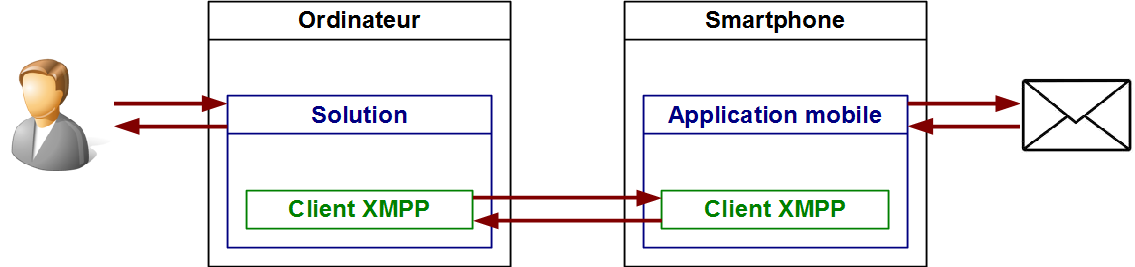
\includegraphics[width=0.9\textwidth]{img/schemaFonctionnement_protocoleTransfert.png}
	\caption{Transfert du message : fonctionnement}
	\label{schemaFonctionnement_protocoleTransfert}
\end{figure}





%%%%%%%%%%%%%%%%%%%%%%%%%%%%%%%%%%%%%%%%%%%%%%%%%%%%%%%%%%%%%%%%%%%%%%%%%%%%%%%%%%%%%%%%%%%%%%%%%%%%
%%%%%%%%%%%%%%%%%%%%%%%%%%%%%%%%%%%%%%%%%%%%%%%%%%%%%%%%%%%%%%%%%%%%%%%%%%%%%%%%%%%%%%%%%%%%%%%%%%%%
%%%%%%%%%%%%%%%%%%%%%%%%%%%%%%%%%%%%%%%%%%%%%%%%%%%%%%%%%%%%%%%%%%%%%%%%%%%%%%%%%%%%%%%%%%%%%%%%%%%%
%%%%%%%%%%%%%%%%%%%%%%%%%%%%%%%%%%%%%%%%%%%%%%%%%%%%%%%%%%%%%%%%%%%%%%%%%%%%%%%%%%%%%%%%%%%%%%%%%%%%
%%%%%%%%%%%%%%%%%%%%%%%%%%%%%%%%%%%%%%%%%%%%%%%%%%%%%%%%%%%%%%%%%%%%%%%%%%%%%%%%%%%%%%%%%%%%%%%%%%%%

\section{Service proposé à l'utilisateur}
\label{Service proposé à l'utilisateur}

%%%%%%%%%%%%%%%%%%%%%%%%%%%%%%%%%%%%%%%%%%%%%%%%%%%%%%%%%%%%%%%%%%%%%%%%%%%%%%%%%%%%%%%%%%%%%%%%%%%%
%%%%%%%%%%%%%%%%%%%%%%%%%%%%%%%%%%%%%%%%%%%%%%%%%%%%%%%%%%%%%%%%%%%%%%%%%%%%%%%%%%%%%%%%%%%%%%%%%%%%
%%%%%%%%%%%%%%%%%%%%%%%%%%%%%%%%%%%%%%%%%%%%%%%%%%%%%%%%%%%%%%%%%%%%%%%%%%%%%%%%%%%%%%%%%%%%%%%%%%%%

\subsection{GTalk}
\label{GTalk}

Google Talk, aussi appelé GTalk, est le client de messagerie instantanée proposé par Google.
Il est disponible à partir de la page web de Gmail, mais aussi en client Windows que l'on peut installer sur son ordinateur (Windows).

Initialement nous voulions utiliser ce client pour envoyer nos SMS pour la simple et bonne raison que de nombreux utilisateurs ont toujours le navigateur web ouvert, ainsi qu'un onglet avec leur boite mail.
De plus, nous voulions nous inspirer d'une solution existante qui utilise GTalk pour l'approfondir et lui ajouter de nouvelles fonctionnalités.

%%%%%%%%%%%%%%%%%%%%%%%%%%%%%%%%%%%%%%%%%%%%%%%%%%%%%%%%%%%%%%%%%%%%%%%%%%%%%%%%%%%%%%%%%%%%%%%%%%%%
%%%%%%%%%%%%%%%%%%%%%%%%%%%%%%%%%%%%%%%%%%%%%%%%%%%%%%%%%%%%%%%%%%%%%%%%%%%%%%%%%%%%%%%%%%%%%%%%%%%%
%%%%%%%%%%%%%%%%%%%%%%%%%%%%%%%%%%%%%%%%%%%%%%%%%%%%%%%%%%%%%%%%%%%%%%%%%%%%%%%%%%%%%%%%%%%%%%%%%%%%

\subsection{Problèmes}
\label{Problèmes}

%%%%%%%%%%%%%%%%%%%%%%%%%%%%%%%%%%%%%%%%%%%%%%%%%%%%%%%%%%%%%%%%%%%%%%%%%%%%%%%%%%%%%%%%%%%%%%%%%%%%

\subsubsection{Parler à soi-même}

Le protocole XMPP autorise et offre la possibilité de s'envoyer des messages instantanés à soi-même si l'expéditeur et le destinataire sont les mêmes comptes.

Cependant GTalk ne le permet pas, pour au moins deux raisons :
\begin{itemize}
	\item Pour envoyer un message à une personne il faut cliquer sur son lien dans la liste des contacts.
	Or notre propre adresse email n'y apparait pas même si l'on s'est ajouté dans nos contacts ;
	\item Gtalk n'affiche pas les messages que l'on s'envoie à soi-même, depuis un autre client XMPP comme une application mobile par exemple.
\end{itemize}

De ce fait, il est donc nécessaire d'utiliser un compte intermédiaire.
On peut ainsi créer un compte spécial qui représentera notre smartphone, et qui sera utilisé uniquement par l'application.
Le fonctionnement global de la solution se résumerait au schéma \ref{schemaFonctionnement_GTalk}.

\begin{figure}[!h]
	\center
	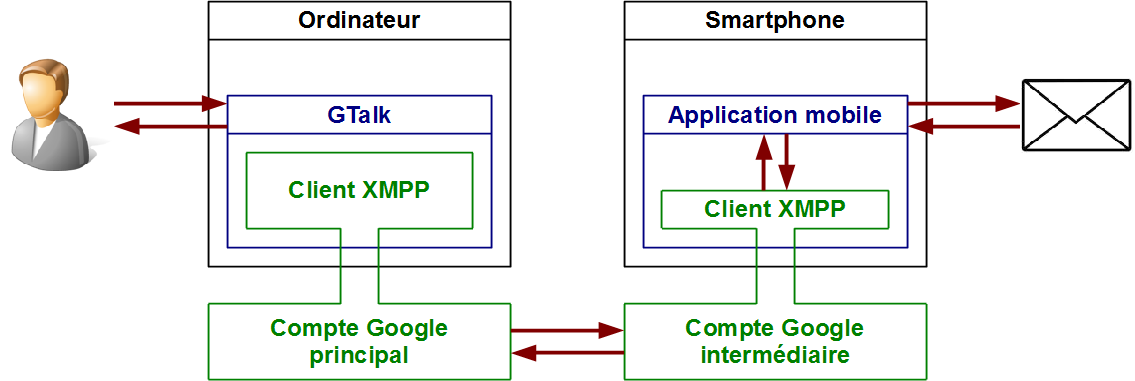
\includegraphics[width=0.9\textwidth]{img/schemaFonctionnement_GTalk.png}
	\caption{GTalk : Utilisation d'un compte intermédiaire}
	\label{schemaFonctionnement_GTalk}
\end{figure}

%%%%%%%%%%%%%%%%%%%%%%%%%%%%%%%%%%%%%%%%%%%%%%%%%%%%%%%%%%%%%%%%%%%%%%%%%%%%%%%%%%%%%%%%%%%%%%%%%%%%

\subsubsection{Praticité}

Pour différencier les SMS que l'utilisateur voudra envoyer et les messages privés qui pourront transiter par le biais du compte intermédiaire, nous voulions imposer une "règle", c'est à dire un format comme par exemple :
\begin{lstlisting}
sms 0123456789 Coucou, comment vas-tu ?
\end{lstlisting}

Mais cela imposera à l'utilisateur de saisir un message correctement formaté.
De plus l'utilisateur devra saisir le numéro de téléphone du destinataire pour pouvoir envoyer le message, ce qui soulèvera les problèmes cités dans la partie \ref{Introduction de l'étude} du rapport.



%%%%%%%%%%%%%%%%%%%%%%%%%%%%%%%%%%%%%%%%%%%%%%%%%%%%%%%%%%%%%%%%%%%%%%%%%%%%%%%%%%%%%%%%%%%%%%%%%%%%
%%%%%%%%%%%%%%%%%%%%%%%%%%%%%%%%%%%%%%%%%%%%%%%%%%%%%%%%%%%%%%%%%%%%%%%%%%%%%%%%%%%%%%%%%%%%%%%%%%%%
%%%%%%%%%%%%%%%%%%%%%%%%%%%%%%%%%%%%%%%%%%%%%%%%%%%%%%%%%%%%%%%%%%%%%%%%%%%%%%%%%%%%%%%%%%%%%%%%%%%%

\subsection{Solution envisagée}

Suite aux inconvénients de GTalk mentionnés précédemment dans la partie \ref{Problèmes}, nous avons dû nous orienter vers une autre solution, indépendante de GTalk.
Plusieurs solutions sont possibles offrant chacune des avantages et des inconvénients.
\\


Le client lourd est un logiciel autonome que l'utilisateur doit "installer" sur son ordinateur.
Son fonctionnement est indépendant de tout serveur, hormis les échanges de données nécessaires aux traitements.
Pour notre projet, l'inconvénient de cette solution est l'obligation d'installation, ce qui peut poser problème lorsque l'on se trouve par exemple au travail ou que l'on utilise un ordinateur qui n'est pas le notre.
\\


Le site web est une application fournie par un serveur distant et accessible depuis n'importe quel navigateur internet.
Aucun programme ne devra être installé car cette solution est totalement indépendante de l'ordinateur de l'utilisateur.
Le seule pré-requis est un accès à internet, qui, quelque soit le type de solution proposé à l'utilisateur (client lourd, client léger, ...), est obligatoire pour l'utilisation du protocole XMPP.
C'est cette solution que nous utiliserons dans ce projet.
\\


Les différentes étapes du fonctionnement du site web est représenté sur le schéma \ref{schemaFonctionnement_siteWeb}
\begin{figure}[!h]
	\center
	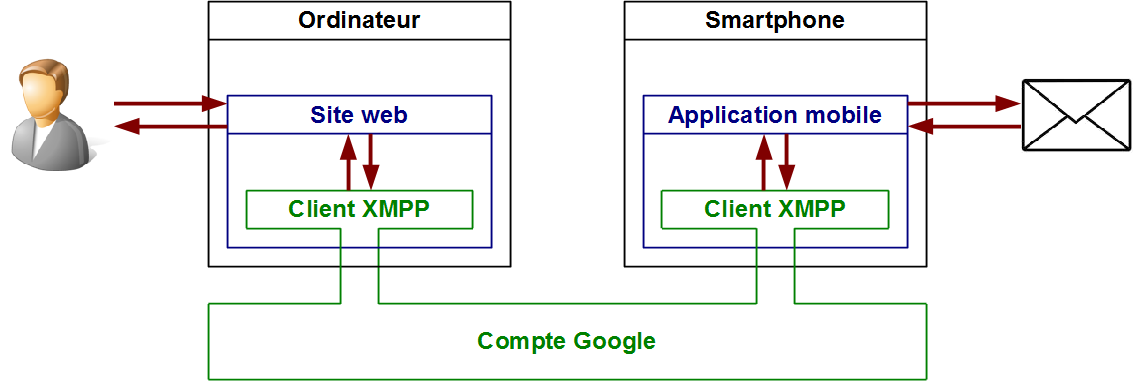
\includegraphics[width=0.9\textwidth]{img/schemaFonctionnement_siteWeb.png}
	\caption{Site web : Réception d'un SMS}
	\label{schemaFonctionnement_siteWeb}
\end{figure}


%%%%%%%%%% Chapitre 3 %%%%%%%%%%
Pour pouvoir transmettre les messages depuis l'utilisateur vers le téléphone portable, nous avons
choisi de mettre en place un site web à l'allure d'un gestionnaire de conversation. 
blablabla

Le fonctionnement de ce projet repose grandement sur la partie qui suit.


%%%%%%%%%%%%%%%%%%%%%%%%%%%%%%%%%%%%%%%%%%%%%%%%%%%%%%%%%%%%%%%%%%%%%%%%%%%%%%%%%%%%%%%%%%%%%%%%%%%%
\subsection{Play Framework 2.0}
%%%%%%%%%%%%%%%%%%%%%%%%%%%%%%%%%%%%%%%%%%%%%%%%%%%%%%%%%%%%%%%%%%%%%%%%%%%%%%%%%%%%%%%%%%%%%%%%%%%%

\subsubsection{primefaces vs playframework}



%%%%%%%%%%%%%%%%%%%%%%%%%%%%%%%%%%%%%%%%%%%%%%%%%%%%%%%%%%%%%%%%%%%%%%%%%%%%%%%%%%%%%%%%%%%%%%%%%%%%
\subsection{Authentification avec OAuth 2.0}
%%%%%%%%%%%%%%%%%%%%%%%%%%%%%%%%%%%%%%%%%%%%%%%%%%%%%%%%%%%%%%%%%%%%%%%%%%%%%%%%%%%%%%%%%%%%%%%%%%%%



%%%%%%%%%%%%%%%%%%%%%%%%%%%%%%%%%%%%%%%%%%%%%%%%%%%%%%%%%%%%%%%%%%%%%%%%%%%%%%%%%%%%%%%%%%%%%%%%%%%%
\subsection{Récupération des contacts google}
%%%%%%%%%%%%%%%%%%%%%%%%%%%%%%%%%%%%%%%%%%%%%%%%%%%%%%%%%%%%%%%%%%%%%%%%%%%%%%%%%%%%%%%%%%%%%%%%%%%%



\subsubsection{récupération des contacts}

\subsubsection{tri et formatage des contacts}

\subsubsection{Google cache}



%%%%%%%%%%%%%%%%%%%%%%%%%%%%%%%%%%%%%%%%%%%%%%%%%%%%%%%%%%%%%%%%%%%%%%%%%%%%%%%%%%%%%%%%%%%%%%%%%%%%
\subsection{Envoi des messages avec les websockets}
%%%%%%%%%%%%%%%%%%%%%%%%%%%%%%%%%%%%%%%%%%%%%%%%%%%%%%%%%%%%%%%%%%%%%%%%%%%%%%%%%%%%%%%%%%%%%%%%%%%%



\subsubsection{websocket}

\subsubsection{notification}



%%%%%%%%%%%%%%%%%%%%%%%%%%%%%%%%%%%%%%%%%%%%%%%%%%%%%%%%%%%%%%%%%%%%%%%%%%%%%%%%%%%%%%%%%%%%%%%%%%%%
\subsection{Design du site}
%%%%%%%%%%%%%%%%%%%%%%%%%%%%%%%%%%%%%%%%%%%%%%%%%%%%%%%%%%%%%%%%%%%%%%%%%%%%%%%%%%%%%%%%%%%%%%%%%%%%

Le design du site est l'un des thèmes que nous avons travaillé pour cette partie la du projet. 
\\
Nous souhaitions initialement avoir une interface simple, sans fioritures car cela nous semblait comme
secondaire. Nous avons donc utilisé deux frameworks pour nous faciliter la tache et accélerer la mise
en place du design.
\\
Nous avons donc tout d'abord choisi "twitter bootstrap" puis nous l'avons couplé au framework "jquery
layout".

\subsubsection{twitter bootstrap}

Twitter bootstrap est un framework web utilisé pour le développement front end. C'est un outil écrit en
Javascript et CSS qui permet de réaliser facilement des interfaces élégantes néanmoins simples. 
\\
Il nous a été utile principalement pour pouvoir concevoir l'affichage des zones d'entrée de textes ou 
encore pour organiser l'affichage des contacts proprement.
\\

\subsubsection{jquery layout}

JQuery layout est aussi un framework web. Contrairement au boostrap de twitter, il nous à permis d'organiser
notre site en plusieurs interfaces distinctes. 
\\
L'utilité de Jquery layout réside dans sa possibilité à fractionner un espace en plusieurs fenetres. Cela permet
de retrouver l'ergonomie et le coté simple et ordonné des logiciels. 
\\
Ce framework très riche nous a donc été très profitable pour pouvoir obtenir une bonne ergonomie sans avoir
à trop passer du temps sur cette partie.
\\\\

Comme le montre l'image \ref{design-final}, le couplage de ces deux frameworks a aidé à obtenir un design simple
mais effiscient. 

\begin{figure}[!h]
	\center
	
\includegraphics[width=13cm]{img/design-final.png}
	\caption{interface finale du site web}
	\label{design-final}
\end{figure}


%\begin{figure}[!h]
%	\center
%	\includegraphics[width=13cm]{img/.png}
%	\caption{}
%	\label{}
%\end{figure}

%%%%%%%%%%%%%%%%%%%%%%%%%%%%%%%%%%%%%%%%%%%%%%%%%%%%%%%%%%%%%%%%%%%%%%%%%%%%%%%%%%%%%%%%%%%%%%%%%%%%
\subsection{Fonctionnement global}
%%%%%%%%%%%%%%%%%%%%%%%%%%%%%%%%%%%%%%%%%%%%%%%%%%%%%%%%%%%%%%%%%%%%%%%%%%%%%%%%%%%%%%%%%%%%%%%%%%%%

Le fonctionnement global du projet sur la plateforme Android est relativement simple. Nous souhaitons
simplement pouvoir utiliser le téléphone portable comme un intermédiaire entre notre site web et le 
correspondant avec qui nous discutons. Pour cela le téléphone fait office de proxy entre les deux 
entités éloignées. Un proxy est un composant qui se place entre un interlocuteur et son auditeur. Le 
proxy sert principalement à relayer l'information d'un élément vers un autre, il sert d'intermédiaire.
Dans notre cas, le proxy s'occupe de recevoir des SMS et de les rediriger vers le site web. 
Réciproquement, il récupère les messages envoyés par le site web et envoie un SMS vers le correspondant
défini  dans le message reçu.



%%%%%%%%%%%%%%%%%%%%%%%%%%%%%%%%%%%%%%%%%%%%%%%%%%%%%%%%%%%%%%%%%%%%%%%%%%%%%%%%%%%%%%%%%%%%%%%%%%%%
\subsection{Création du service}
%%%%%%%%%%%%%%%%%%%%%%%%%%%%%%%%%%%%%%%%%%%%%%%%%%%%%%%%%%%%%%%%%%%%%%%%%%%%%%%%%%%%%%%%%%%%%%%%%%%%

Les applications fonctionnant sous Android régissent par un principe simple, celui des "activités".
Pour simplifier, une activité représente une fonctionnalité graphique d'une application. Par exemple,
lorsqu'une application est ouverte, on tombe sur un menu avec différentes possibilités d'actions 
qui nous sont offertes. Le menu représente donc ici une activité.
\\


Il faut savoir qu’une activité, lorsqu'elle est active, occupe le système qui attend des événements.
Si l'utilisateur ne fait rien alors que le menu est affiché, le système peut s'occuper d'autres 
tâches annexes. Si en revanche l'utilisateur navigue dans le menu, alors l'activité est considérée
comme en fonctionnement et bloque toutes autres opérations non relatives à l'application exécutée.
\\


Dans le cadre de notre application, nous devons à son lancement, effectuer une série d'opérations 
afin de mettre l'application en fonctionnement. Cela consiste notamment, à vérifier l'état de la 
connectivité internet, récupérer les identifiants et se connecter sur le service GTalk. Ces 
opérations rendent le système bloquant durant leur exécution. Cela n'est pas un problème lorsque la 
connection s'effectue sans erreur. Le traitement durant moins d'une seconde, le système n'est pas
gravement impacté. En revanche, si une erreur intervient, le programme va alors essayer de la résoudre.
Cela n'est pas concevable. En effet, une perte soudaine de réseau pourrait par exemple mettre 
l'application dans un état de recherche ce qui est potentiellement très lent. Cette situation rendrait
le terminal complètement bloqué durant la recherche. 

Ce comportement n'étant pas souhaitable, nous avons dû trouver une solution pour pouvoir outrepasser ce blocage.
\\


Nous avons alors utilisé le concept Android de "services". Celui-ci consiste à exécuter une fonctionnalité 
de manière asynchrone. Le service n'impacte pas le système, au contraire il fonctionne avec lui. 
 
\begin{figure}[!h]
  \center
  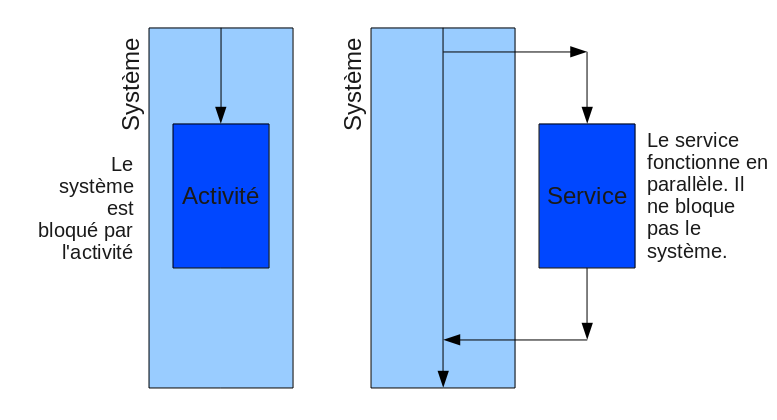
\includegraphics[width=13cm]{img/fonctionnement-des-services-android.png}
  \caption{Fonctionnement d'un service Android}
  \label{fonctionnement-des-services-android}
\end{figure}

Comme montré dans la figure \ref{fonctionnement-des-services-android}, le service n'est pas  bloquant. 
Lors de son exécution, le système continue de fonctionner sur d'autres tâches en paire avec le service lancé.
\\


Dans notre cas, le service sert à deux tâches principales. Tout d'abord il va configurer l'authentification
de l'utilisateur sur GTalk. Ensuite il va simplement se mettre en attente d'événements et le cas échéant, 
traiter ce même événement.



%%%%%%%%%%%%%%%%%%%%%%%%%%%%%%%%%%%%%%%%%%%%%%%%%%%%%%%%%%%%%%%%%%%%%%%%%%%%%%%%%%%%%%%%%%%%%%%%%%%%
\subsection{Authentification sur GTalk}
%%%%%%%%%%%%%%%%%%%%%%%%%%%%%%%%%%%%%%%%%%%%%%%%%%%%%%%%%%%%%%%%%%%%%%%%%%%%%%%%%%%%%%%%%%%%%%%%%%%%

Pour pouvoir converser avec le site web, l'application a besoin de s'authentifier auprès du service
GTalk. Pour cela, nous sommes passés par deux étapes. 
\\


Initialement, nous utilisions la méthode classique d'authentification. Lorsque l'utilisateur lance 
l'application, celle-ci lui demande de rentrer ses identifiant et mot de passe. Cela effectué, 
l'application se charge de se connecter et de s'authentifier sur les serveurs GTalk en utilisant les
paramètres rentrés par l'utilisateur.

Cette solution est la plus simple à implémenter mais n'est malheureusement pas la plus agréable
à utiliser ni la plus sure. Nous forçons en effet l'utilisateur à rentrer ses identifiants ce qui 
pourrait paraître légitime mais reste contraignant pour l'utilisateur. Celui-ci ne sait pas ce que 
nous faisons avec son mot de passe. Une application malveillante pourrait récupérer les identifiants
et s'en servir à des fins illégales. Dans notre cas, même si nous n'avions aucune mauvaise intention,
nous ne pouvons demander aux utilisateurs de nous faire confiance. Nous avons donc opté pour une 
deuxième solution, l'identification avec OAuth 2.0.
\\


Comme détaillé dans la partie \ref{Authentification avec OAuth 2.0}, OAuth permet de réaliser des actions en agissant à la place de l'utilisateur. 
Ici nous souhaitions simplement utiliser le compte GTalk de l'utilisateur sans que celui-ci ai à rentrer
ses identifiants. 

Contrairement à l'authentification sur le site web, l'authentification sur une plateforme Android est
théoriquement plus simple. En effet, une fois que l'utilisateur a donné son accord, le serveur 
d'authentification de Google va directement envoyer le token d'authentification. Il n'y a alors pas 
besoin d'effectuer une deuxième étape pour récupérer ce dernier comme le montre le diagramme 
\ref{obtention-token-avec-android}.

%%%%%%%%%%%%%%%%%%%%%%%%%%%%
%title Envoi d'un SMS
 
%Utilisateur->Application: délégation de l'authentification
%Application->Serveur Google: requête pour un token d'authentification
%Serveur Google->Application: token d'authentification
%Application->serveur GTalk: authentification(token)
%serveur GTalk->Application: authentification validé
%%%%%%%%%%%%%%%%%%%%%%%%%%%%

\begin{figure}[!h]
  \center
  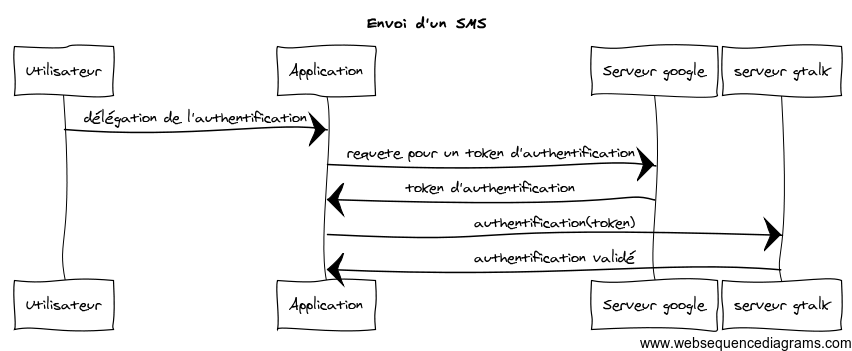
\includegraphics[width=15cm]{img/obtention-token-avec-android.png}
  \caption{Procédure d'obtention d'un token avec un appareil Android}
  \label{obtention-token-avec-android}
\end{figure}

% utilisation de aSmack ?
Néanmoins, une des difficultés d'implémenter ce protocole est que la librairie de gestion de compte
XMPP pour Android dénommée Asmack est différente de celle utiliser pour le site web. Asmack est un fork 
de la librairie Smack pour Android et est l'unique librairie gérant les comptes XMPP présente sur
Android. Ne souhaitant pas ré-implémenter toutes les fonctionnalités présentes dans celle-ci, nous avons
choisi de l'utiliser. Malheureusement, les différences entre les deux librairies nous ont empêché de 
ré-implémenter notre précédent travail effectué pour le site web qui était fonctionnel. 

Le langage Java fonctionne sur une machine virtuelle. Celle-ci contient des fonctionnalités basique sur
lesquelles le langage peut s'appuyer. Dalvik, la machine virtuelle pour Java présente sur Android n'est 
pas exactement la même que la machine virtuelle basique. En effet, pour des soucis de rapidité et de 
légèreté, certaines parties de Dalvik ont été réécrites pour en faire une machine virtuelle plus adaptée
aux plateformes mobiles.

Smack a été développé sur la machine virtuelle Java basique tandis que Asmack a été développé sur Dalvik.
Cette différence implique des changements quant aux fonctionnements de celles-ci.

Finalement, en ré-implémentant certaines fonctionnalités, nous avons réussi à nous authentifier avec OAuth.
\\


Authentifier un utilisateur via OAuth2.0 sur Android a été un réel challenge. Il nous a fallu comprendre 
et trouver des équivalences au fonctionnement de Smack.



%%%%%%%%%%%%%%%%%%%%%%%%%%%%%%%%%%%%%%%%%%%%%%%%%%%%%%%%%%%%%%%%%%%%%%%%%%%%%%%%%%%%%%%%%%%%%%%%%%%%
\subsection{Envoi et réception d'un SMS}
%%%%%%%%%%%%%%%%%%%%%%%%%%%%%%%%%%%%%%%%%%%%%%%%%%%%%%%%%%%%%%%%%%%%%%%%%%%%%%%%%%%%%%%%%%%%%%%%%%%%

\subsubsection{Réception d'un SMS}

Une fois authentifié, nous souhaitons pouvoir utiliser notre téléphone comme proxy. Notre application
doit en effet servir d'intermédiaire entre le site web et un correspondant. Pour cela elle doit tout
d'abord surveiller l'arrivée de nouveaux messages. 
\\


Google autorisent la surveillance du comportement du téléphone sur Android, permettant de réagir lors de différents événements.
Dans notre cas nous avons pu utiliser le principe de "Broadcast Receiver" du système. 
Un broadcast receiver est un outil qui permet de rendre une application consciente de son environnement.
Cela permet généralement à l'application qui l'utilise d'être prévenue lors de nouvelles notifications ou 
d'un comportement particulier du téléphone.
Son fonctionnement est simple : il permet de s'enregistrer auprès du téléphone qui maintient une base de donnée des membres à avertir lors d'un changement particulier.

\begin{figure}[!h]
  \center
  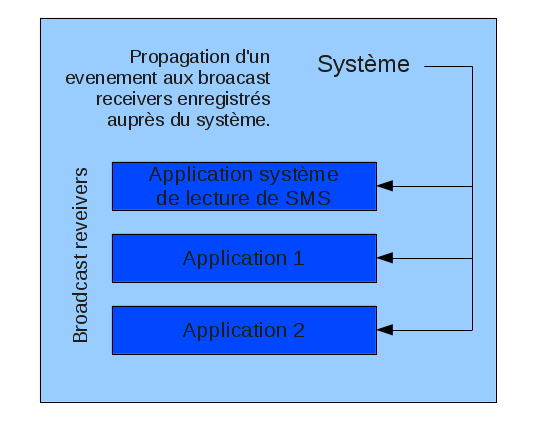
\includegraphics[width=12cm]{img/broadcast-receivers.png}
  \caption{Android : fonctionnement des broadcasts receivers}
  \label{broadcast-receivers}
\end{figure}

Le schéma \ref{broadcast-receivers} permet de voir le système du téléphone qui contient les différents broadcast receiver à avertir en cas de nouveaux messages. Ici l'application de rédaction de SMS ainsi que deux autres 
applications seront averties.

Dans notre cas, nous nous en sommes servis pour d'une part être avertis de l'arrivée de nouveaux SMS et d'autre part pour pouvoir récupérer le dit message et le traiter.


\subsubsection{Envoi d'un SMS}

L'envoi quant à lui est beaucoup plus trivial. Android met à disposition un outil permettant d'envoyer
des messages.

% développer ?



%%%%%%%%%%%%%%%%%%%%%%%%%%%%%%%%%%%%%%%%%%%%%%%%%%%%%%%%%%%%%%%%%%%%%%%%%%%%%%%%%%%%%%%%%%%%%%%%%%%%
%%%%%%%%%%%%%%%%%%%%%%%%%%%%%%%%%%%%%%%%%%%%%%%%%%%%%%%%%%%%%%%%%%%%%%%%%%%%%%%%%%%%%%%%%%%%%%%%%%%%
%%%%%%%%%%%%%%%%%%%%%%%%%%%%%%%%%%%%%%%%%%%%%%%%%%%%%%%%%%%%%%%%%%%%%%%%%%%%%%%%%%%%%%%%%%%%%%%%%%%%

\subsection{Fonctionnement}

%%%%%%%%%%%%%%%%%%%%%%%%%%%%%%%%%%%%%%%%%%%%%%%%%%%%%%%%%%%%%%%%%%%%%%%%%%%%%%%%%%%%%%%%%%%%%%%%%%%%

\subsubsection{Globalité}

Le fonctionnement global de notre application est relativement simple.
Elle a été tout d'abord implémentée de manière à répondre aux besoins du projet et être fonctionnelle pour donner une première version.

Lors de la réception d'un SMS sur le smartphone l'application va tout d'abord récupérer le contenu du message ainsi que son auteur.
Puis les données sont être encapsulée dans un message au format JSON.
Enfin le message est envoyé vers le webservice grâce à GTalk, qui s'occupera de notifier à l'utilisateur l'arrivée d'un nouveau message.

\begin{figure}[!h]
  \center
  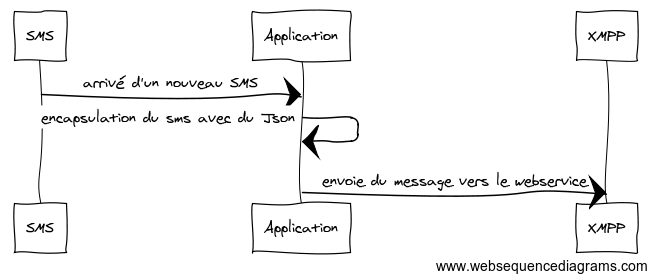
\includegraphics[width=12cm]{img/encapsulation-sms.png}
  \caption{Traitements lors de la réception d'un SMS}
  \label{encapsulation-sms}
\end{figure}

Lors de la réception d'un nouveau message XMPP la méthode est l'inverse de celle de la réception d'un SMS.
L'application va dé désencapsuler le message XMPP pour y récupérer l'information utile.
Cela fait, notre application va ensuite envoyer le SMS au destinataire.

%%%%%%%%%%%%%%%%%%%%%%%%%%%%%%%%%%%%%%%%%%%%%%%%%%%%%%%%%%%%%%%%%%%%%%%%%%%%%%%%%%%%%%%%%%%%%%%%%%%%

\subsubsection{Architecture}

Dans le cadre de notre projet, nous n'avions comme but, l'envoi de SMS à partir du webservice seulement.
Lors de la réception d'un message XMPP, nous souhaitions pouvoir réagir différemment en fonction du contenu du message.
Notre travail respectait donc ce principe mais ne permettait aucune évolutivité.

A supposer qu'un tiers soit intéressé par la communication entre le webservice et le téléphone par 
l'intermédiaire de XMPP, mais que son but ne soit pas d'envoyer de simple SMS, nous avons implémenté une
architecture permettant de rajouter facilement de nouvelles fonctionnalités. Pour donner des exemples, 
un utilisateur pourrait décider d'implémenter une fonctionnalité lui permettant de déclencher la capture
de photos de son téléphone à partir du webserver.
 
Pour permettre cette évolutivité, nous avons réalisé une architecture qui s'adapte automatiquement en
fonction des messages reçus. Il s'agit ici des patrons de conceptions fabrique et stratégie. 


\Jparagraph{Pattern stratégie}

Le patron de stratégie est un patron de conception de type comportemental.
Il permet d'adopter dynamiquement un comportement particulier en fonction des conditions de son exécution.
Concrètement, quelque soit la classe implémentant l'interface de base, l'exécution d'un algorithme s'effectue simplement depuis une seule méthode.
Le schéma \ref{pattern_strategie} décrit le fonctionnement du modèle.

\begin{figure}[H]
  \center
  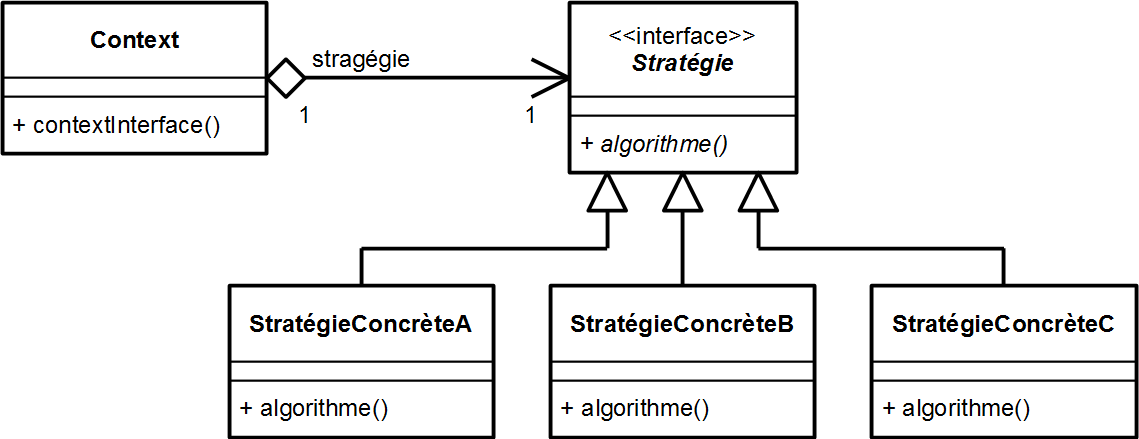
\includegraphics[width=12cm]{img/pattern_strategie.png}
  \caption{Pattern stratégie : diagramme UML}
  \label{pattern_strategie}
\end{figure}

Dans notre cas, il permet de créer différents types de stratégies qui pourront potentiellement être utilisés.
Notre projet ne contient pour l'instant que les stratégies "envoi de SMS" et "envoi de messages XMPP", mais avec cette architecture il est possible de rajouter d'autres stratégies, comme par exemple l'extinction du téléphone ou encore l'envoi d'un email par exemple.
\\


\Jparagraph{Pattern fabrique}

L'avantage du pattern stratégie est qu'il permet de regrouper les algorithmes à exécuter dans des classes séparées plutôt que de le mélanger dans du code différent.
Mais son inconvénient réside dans le fait qu'il est nécessaire d'effectuer un test sur le type d'algorithme à exécuter à chaque endroit où l'on doit instancier les stratégies.

Le pattern fabrique permet de palier à ce problème en définissant les règles d'instanciation des différentes stratégies.
Ainsi les différents tests ne se retrouvent pas dupliqués à chaque parties du code, mais regroupé dans une classe qui se chargera de définir la stratégie à appliquer en fonction des données qu'on lui transmet.
Le schéma \ref{pattern_fabrique} représente le diagramme de classe du pattern fabrique.
 
\begin{figure}[H]
  \center
  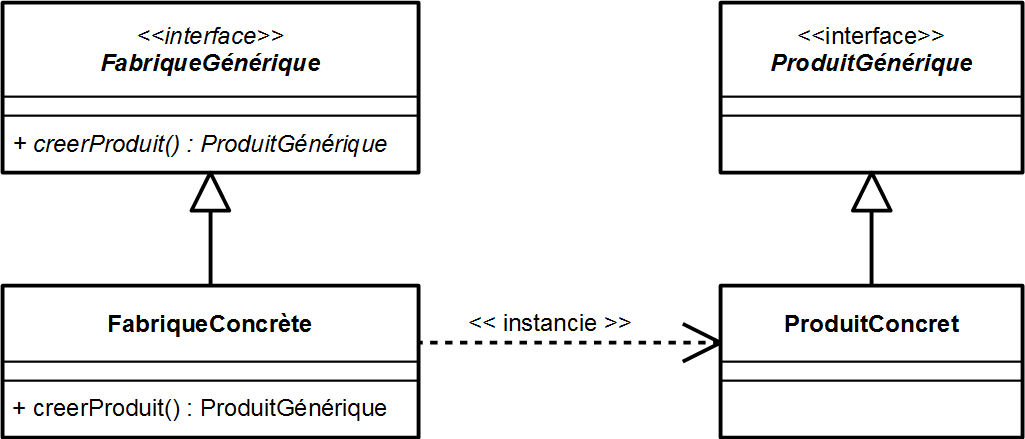
\includegraphics[width=10cm]{img/pattern_fabrique.png}
  \caption{Pattern fabrique : diagramme UML}
  \label{pattern_fabrique}
\end{figure}
 
Dans notre cas la fabrique va analyser chaque nouveau message.
En fonction de leurs contenus elle devra décider d'une stratégie.
\\


\Jparagraph{Ajout de fonctionnalités}

\begin{figure}[!h]
  \center
  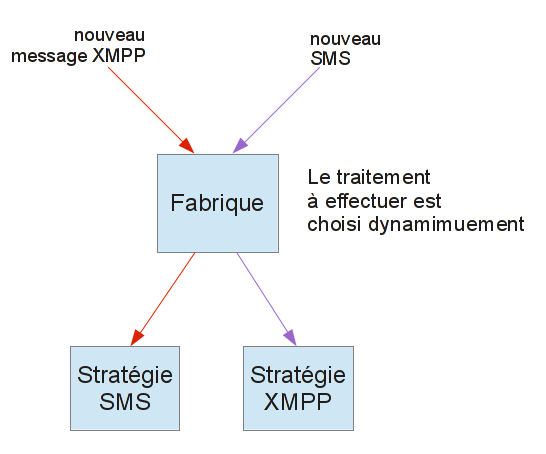
\includegraphics[width=10cm]{img/fonctionnement-strategie-factorie.png}
  \caption{Pattern fabrique : fonctionnement}
  \label{fonctionnement-strategie-factorie}
\end{figure}

La figure \ref{fonctionnement-strategie-factorie} montre le fonctionnement du projet lors de l'arrivée d'un
nouveau message (SMS ou XMPP).
L'intérêt principal de ce pattern est l'évolutivité qu'il apporte.
Le choix dynamique à l'exécution de la stratégie à un intérêt pour le développeur.
En effet, celui-ci n'a plus besoin de se soucier de l'implémentation du choix de la stratégie ni de son exécution.

L'ajout d'une fonctionnalité ne se fait plus dans chaque partie du code source, mais en définissant une nouvelle stratégie (classe représentative) puis en ajoutant sa définition dans la fabrique.

%%%%%%%%%%%%%%%%%%%%%%%%%%%%%%%%%%%%%%%%%%%%%%%%%%%%%%%%%%%%%%%%%%%%%%%%%%%%%%%%%%%%%%%%%%%%%%%%%%%%
%%%%%%%%%%%%%%%%%%%%%%%%%%%%%%%%%%%%%%%%%%%%%%%%%%%%%%%%%%%%%%%%%%%%%%%%%%%%%%%%%%%%%%%%%%%%%%%%%%%%
%%%%%%%%%%%%%%%%%%%%%%%%%%%%%%%%%%%%%%%%%%%%%%%%%%%%%%%%%%%%%%%%%%%%%%%%%%%%%%%%%%%%%%%%%%%%%%%%%%%%

\subsection{Objective-C et Xcode}

Objective-C est un langage de programmation orienté objet et réflexif.
Compilé et libre, il hérite du langage C (comme le C++) en lui rajoutant l'aspect objet, ce qui lui permet d'être interfacé avec du Langage C ou du C++.
Principalement présent sur les systèmes d'exploitation des produits de la marque Apple (OS X et iOS), ce langage est multi-plateforme.
\\


Xcode est l'environnement de développement intégré (EDI, ou IDE pour Integrated Development Environment) pour Mac OS X.
Il permet le développement d'application en Langage C, C++ et bien évidemment en Objective-C pour OS X ou iOS.
C'est un IDE très complet qui comporte un éditeur de texte, un débogueur, un compilateur, un gestionnaire de projet et de version, un gestionnaire de documents pour la documentation, et d'autres outils facilitant le développement.
\\



%%%%%%%%%%%%%%%%%%%%%%%%%%%%%%%%%%%%%%%%%%%%%%%%%%%%%%%%%%%%%%%%%%%%%%%%%%%%%%%%%%%%%%%%%%%%%%%%%%%%
%%%%%%%%%%%%%%%%%%%%%%%%%%%%%%%%%%%%%%%%%%%%%%%%%%%%%%%%%%%%%%%%%%%%%%%%%%%%%%%%%%%%%%%%%%%%%%%%%%%%
%%%%%%%%%%%%%%%%%%%%%%%%%%%%%%%%%%%%%%%%%%%%%%%%%%%%%%%%%%%%%%%%%%%%%%%%%%%%%%%%%%%%%%%%%%%%%%%%%%%%

\subsection{Les frameworks}

Un \textit{framework} est un ensemble d'outils et de composants structurels qui permettent le développement de logiciels ou de sites web.

Apple propose de nombreux frameworks permettant de simplifier la tâche des développeurs.
Ils respectent les \textit{design patterns} pour structurer l'agencement des différents objets, comme par exemple l'architecture MVC des interfaces graphiques.
Ces frameworks font la force des applications iOS car ils permettent d'interagir très facilement avec les composants des terminaux, comme par exemple le gyroscope, l'appareil photo, l'envoi de mail, l'affichage d'une carte, ...
\\


Pour pouvoir publier des applications sur l'Apple Store, il est nécessaire d'utiliser des frameworks dits "publics" : documentés et approuvés.
Cette politique très ferme d'Apple permet d'éviter toute faille de sécurité et permet de proposer des applications sûres aux utilisateurs.
\\


Les frameworks d'Apple sont composés de deux parties : le framework dit "public" et le framework dit "privé".

Pour pouvoir publier des applications sur l'Apple Store, il est nécessaire d'utiliser des frameworks publics : documentés et approuvés.
Cette politique très ferme d'Apple permet d'éviter toute faille de sécurité et permet de proposer des applications sûres aux utilisateurs.

Les frameworks privés ne sont pas directement utilisables comme les publics.
En effet, les fichiers d'entête (headers ".h") n'incluent pas les prototypes des fonctions et méthodes privées, et le programme n'est pas compilable.
Pour cela, il est nécessaire d'inclure les fichiers d'entête privés qui permettront la compilation du programme.
\\



%%%%%%%%%%%%%%%%%%%%%%%%%%%%%%%%%%%%%%%%%%%%%%%%%%%%%%%%%%%%%%%%%%%%%%%%%%%%%%%%%%%%%%%%%%%%%%%%%%%%
%%%%%%%%%%%%%%%%%%%%%%%%%%%%%%%%%%%%%%%%%%%%%%%%%%%%%%%%%%%%%%%%%%%%%%%%%%%%%%%%%%%%%%%%%%%%%%%%%%%%
%%%%%%%%%%%%%%%%%%%%%%%%%%%%%%%%%%%%%%%%%%%%%%%%%%%%%%%%%%%%%%%%%%%%%%%%%%%%%%%%%%%%%%%%%%%%%%%%%%%%

\subsection{Manipulation des SMS}

%%%%%%%%%%%%%%%%%%%%%%%%%%%%%%%%%%%%%%%%%%%%%%%%%%%%%%%%%%%%%%%%%%%%%%%%%%%%%%%%%%%%%%%%%%%%%%%%%%%%

\subsubsection{Envoi de SMS}

Apple n'autorise l'envoi de SMS qu'en utilisant leur framework officiel \textit{MessageUI}.
Lorsque l'application désire envoyer le SMS une fenêtre s'affiche et l'utilisateur doit confirmer l'envoi en appuyant sur le bouton prévu à cet effet.
Cette méthode ne peut pas être utilisée dans ce projet, car l'application mobile fonctionne en tâche de fond et doit envoyer les SMS de manière automatique.

Cependant l'utilisation du framework privé \textit{CoreTelephony} le permet.
L'envoi de SMS peut ainsi se faire grâce à une ligne de code et de manière totalement automatique.
\\

%%%%%%%%%%%%%%%%%%%%%%%%%%%%%%%%%%%%%%%%%%%%%%%%%%%%%%%%%%%%%%%%%%%%%%%%%%%%%%%%%%%%%%%%%%%%%%%%%%%%

\subsubsection{Réception de SMS}

La réception des SMS se décomposent en deux étapes : l'événement de réception, puis la lecture.

\paragraph{Événement de réception -}
Le système envoie des notifications lors des appels ou de la réception des SMS.
Pour que notre programme reçoive ces notifications il est nécessaire de définir une fonction qui sera appelée lorsque ces événements seront émis.
Cela se fait grâce à la fonction \lstinline{CTTelephonyCenterAddObserver()} dans laquelle un des paramètres correspond à la fonction appelée.

% TODO: jailbreak ?


\paragraph{Lecture des SMS -}
Les SMS sont stockés dans une base de données SQLite dont le fichier est \lstinline{/private/var/mobile/Library/SMS/sms.db} dans le répertoire du terminal.
Pour parcourir les messages il est nécessaire d'effectuer des requêtes SQL, comme dans n'importe quelle base de données.

Mais un problème critique : il est impossible d'accéder à ce fichier depuis une application.
En effet, les application iOS fonctionnent dans une \textit{Sandbox}, qui est un environnement virtuel clos permettant la protection contre les processus malveillants.

Malheureusement aucune solution d'accès au fichier n'a été trouvée pour le moment.
En attendant de trouver une solution, nous avons copié le fichier dans un répertoire accessible pour effectuer les différents tests de lecture, et la fonction permettant la lecture des SMS renvoie des données "statiques" pour valider le fonctionnement de l'application.
\\



%%%%%%%%%%%%%%%%%%%%%%%%%%%%%%%%%%%%%%%%%%%%%%%%%%%%%%%%%%%%%%%%%%%%%%%%%%%%%%%%%%%%%%%%%%%%%%%%%%%%
%%%%%%%%%%%%%%%%%%%%%%%%%%%%%%%%%%%%%%%%%%%%%%%%%%%%%%%%%%%%%%%%%%%%%%%%%%%%%%%%%%%%%%%%%%%%%%%%%%%%
%%%%%%%%%%%%%%%%%%%%%%%%%%%%%%%%%%%%%%%%%%%%%%%%%%%%%%%%%%%%%%%%%%%%%%%%%%%%%%%%%%%%%%%%%%%%%%%%%%%%

\subsection{Les messages XMPP}

ICI
\\


%%%%%%%%%% Chapitre 3 %%%%%%%%%%
\cleardoublepage



\chapter{Résultats - Discussion}

Nous ayons pu terminer le projet dans les temps seuleument, meme si celui-ci est aujourd'hui fonctionnel,
il persiste encore certains problèmes. Concernant tout d'abord les applications mobiles, certaines 
contraintes imposés par les systèmes d'exploitations nous ont empechés de construire une application 
qui marche sur n'importe quel téléphone.
\\
Au vu des des techniques employés, il nous parait peu probable de pouvoir publier aucune des
deux applications sur les "markets" officiels de Apple et Google.
\\\\

En ce qui concerne le site web, les résultats sont probants. Néanmoins, plusieurs fonctionnalités
auquels nous avions pensé manquent. Nous discuterons principalement des possibilités d'évolutions du 
produit.

%%%%%%%%%%%%%%%%%%%%%%%%%%%%%%%%%%%%%%%%%%%%%%%%%%%%%%%%%%%%%%%%%%%%%%%%%%%%%%%%%%%%%%%%%%%%%%%%%%%%
%%%%%%%%%%%%%%%%%%%%%%%%%%%%%%%%%%%%%%%%%%%%%%%%%%%%%%%%%%%%%%%%%%%%%%%%%%%%%%%%%%%%%%%%%%%%%%%%%%%%
%%%%%%%%%%%%%%%%%%%%%%%%%%%%%%%%%%%%%%%%%%%%%%%%%%%%%%%%%%%%%%%%%%%%%%%%%%%%%%%%%%%%%%%%%%%%%%%%%%%%
%%%%%%%%%%%%%%%%%%%%%%%%%%%%%%%%%%%%%%%%%%%%%%%%%%%%%%%%%%%%%%%%%%%%%%%%%%%%%%%%%%%%%%%%%%%%%%%%%%%%
%%%%%%%%%%%%%%%%%%%%%%%%%%%%%%%%%%%%%%%%%%%%%%%%%%%%%%%%%%%%%%%%%%%%%%%%%%%%%%%%%%%%%%%%%%%%%%%%%%%%

\section{Site web}

- Réception de SMS de personnes qui ne sont pas dans nos contacts

- Peut-être charger la liste des anciens contacts
\\





%%%%%%%%%%%%%%%%%%%%%%%%%%%%%%%%%%%%%%%%%%%%%%%%%%%%%%%%%%%%%%%%%%%%%%%%%%%%%%%%%%%%%%%%%%%%%%%%%%%%
%%%%%%%%%%%%%%%%%%%%%%%%%%%%%%%%%%%%%%%%%%%%%%%%%%%%%%%%%%%%%%%%%%%%%%%%%%%%%%%%%%%%%%%%%%%%%%%%%%%%
%%%%%%%%%%%%%%%%%%%%%%%%%%%%%%%%%%%%%%%%%%%%%%%%%%%%%%%%%%%%%%%%%%%%%%%%%%%%%%%%%%%%%%%%%%%%%%%%%%%%
%%%%%%%%%%%%%%%%%%%%%%%%%%%%%%%%%%%%%%%%%%%%%%%%%%%%%%%%%%%%%%%%%%%%%%%%%%%%%%%%%%%%%%%%%%%%%%%%%%%%
%%%%%%%%%%%%%%%%%%%%%%%%%%%%%%%%%%%%%%%%%%%%%%%%%%%%%%%%%%%%%%%%%%%%%%%%%%%%%%%%%%%%%%%%%%%%%%%%%%%%

\section{Applications mobiles}

%%%%%%%%%%%%%%%%%%%%%%%%%%%%%%%%%%%%%%%%%%%%%%%%%%%%%%%%%%%%%%%%%%%%%%%%%%%%%%%%%%%%%%%%%%%%%%%%%%%%
%%%%%%%%%%%%%%%%%%%%%%%%%%%%%%%%%%%%%%%%%%%%%%%%%%%%%%%%%%%%%%%%%%%%%%%%%%%%%%%%%%%%%%%%%%%%%%%%%%%%
%%%%%%%%%%%%%%%%%%%%%%%%%%%%%%%%%%%%%%%%%%%%%%%%%%%%%%%%%%%%%%%%%%%%%%%%%%%%%%%%%%%%%%%%%%%%%%%%%%%%

\subsection{Androïd}

\subsubsection{Problèmes rencontrés}

De nombreux problèmes sont venus troubler l'avancement du projet. Nous avons toujours essayer de les
résoudres de la manière la plus effisciente qui soit. Seulement, il nous est arrivé de bloquer sur des
parties pour lesquelles aucune solutions propres n'étaient réalisable. Nous avons alors du appliquer 
des manipulations qui empecheront ce projet d'etre un projet considéré comme stable dans un environnement
grand public.

\paragraph{Message Gtalk}

Ce problème concerne autant l'architecture iOS que Android. 
\\
Le choix de prendre GTalk comme moyen de communication n'était pas sans conséquences. En effet, il nous
est apparu impossible d'avoir une gestion fine de GTalk.
\\\\
Lors de l'envoi d'un message XMPP d'un compte A vers un compte B, toutes les interfaces de connexions
de B recevront le message. GTalk ne fait malheuresement pas exception de plus dans notre cas, l'envoi
se fait d'un compte A vers le meme compte A. En pratique cela revient à recevoir et traiter beaucoup de
message inutiles.
\\\\
Premièrement, en ce qui concerne le traitement, les applications étant connectés sur leur compte GTalk, 
le message envoyé sera immédiatement reçu par l'application. Celle-ci bien heureusement filtrera les 
messages qui ne lui sont pas destinés. 

\begin{figure}[!h]
	\center
	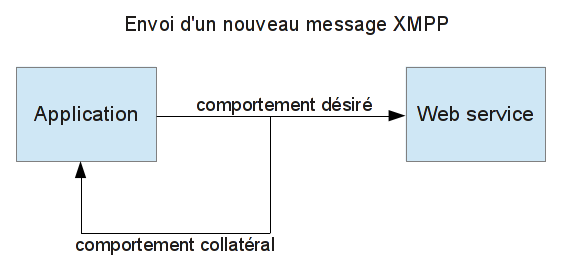
\includegraphics[width=12cm]{img/boucle-envoi-xmpp.png}
	\caption{Création d'une boucle lors de l'envoi d'un message XMPP}
	\label{boucle-envoi-xmpp}
\end{figure}

Comme le montre l'image \ref{boucle-envoi-xmpp}, une boucle se crée. Dans les faits, elle ne causera jamais de problème 
néanmoins c'est un comportement qui n'était pas désiré et qu'on aurait souhaitait évité.
\\\\
Deuxièmement, l'utilisation de GTalk était problèmatique. L'impossibilité de gérer finement GTalk fait que
tous les messages que nous envoyons, que ce soit depuis le téléphone ou bien depuis le site web étaient
aussi redirigés vers les outils utilisant GTalk.
\\
En pratique, cela impliquait de recevoir des messages au format JSon sur plusieurs lieux indésirés.

\begin{figure}[!h]
	\center
	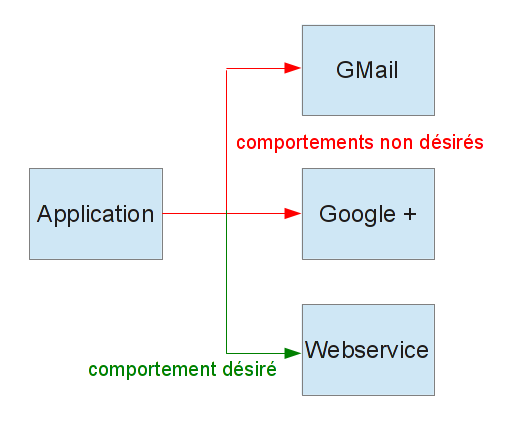
\includegraphics[width=10cm]{img/broadcast-xmpp.png}
	\caption{destinataires lors d'un envoi d'un message XMPP}
	\label{broadcast-xmpp}
\end{figure}

Comme le montre le schéma \ref{broadcast-xmpp}, lors de l'envoi d'un message XMPP origenellement destiné uniquement
à une application ou au webservice, c'est tous l'environnement qui reçoit et affiche le nouveaux messages.
Le résultat est montré dans l'image \ref{message-xmpp-json-gmail}, un message XMPP au format JSon. 
	
\begin{figure}[!h]
	\center
	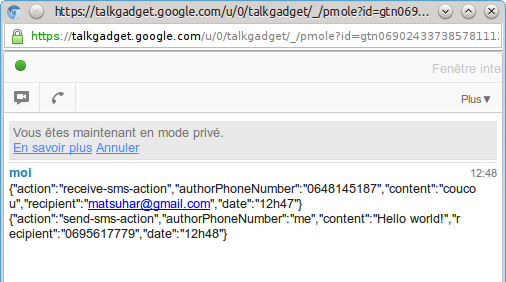
\includegraphics[width=10cm]{img/message-xmpp-json-gmail.png}
	\caption{message XMPP au format JSON reçu avec GTalk}
	\label{message-xmpp-json-gmail}
\end{figure}

\paragraph{Limite des SMS}

\\



%%%%%%%%%%%%%%%%%%%%%%%%%%%%%%%%%%%%%%%%%%%%%%%%%%%%%%%%%%%%%%%%%%%%%%%%%%%%%%%%%%%%%%%%%%%%%%%%%%%%
%%%%%%%%%%%%%%%%%%%%%%%%%%%%%%%%%%%%%%%%%%%%%%%%%%%%%%%%%%%%%%%%%%%%%%%%%%%%%%%%%%%%%%%%%%%%%%%%%%%%
%%%%%%%%%%%%%%%%%%%%%%%%%%%%%%%%%%%%%%%%%%%%%%%%%%%%%%%%%%%%%%%%%%%%%%%%%%%%%%%%%%%%%%%%%%%%%%%%%%%%

\subsection{iOS}

Impossible de lire les contacts...
\\


%%%%%%%%%% Conclusion %%%%%%%%%%
 \cleardoublepage

 

\chapter*{Conclusion}

\addcontentsline{toc}{chapter}{Conclusion}

 

Ce projet avait pour objectif de trouver et développer une solution permettant aux utilisateurs d'envoyer des SMS depuis un ordinateur.
De plus notre cahier des charges imposait une gestion fine des contacts pour obtenir une solution simple et pratique.

Notre première solution remplie entièrement le cahier des charges en proposant une première solution fonctionnelle à l'utilisateur. 
Du côté des applications mobiles qui font office d'intermédiaire entre le site web et le correspondant, le bilan est mitigé. L'application mobile Android est terminée et maintenable grâce à son architecture, alors que l'application iOS est bloquée pour des raisons de sécurité.
Néanmoins, aucune des deux applications n'est aujourd'hui potentiellement publiable sur les markets officiels de Apple et Google. Les techniques employées pour leur fonctionnement les rendent incompatibles avec les politiques mises en place par les responsables des systèmes d'exploitations.
Le site web, quant à lui, propose une première version fonctionnelle pour l'utilisateur. L'utilisateur pourra alors se connecter sur le site web avec ses identifiants Google, verra ses contacts s'afficher et pourra discuter avec chacun d'entre eux à condition d'avoir installé et activé l'application mobile iOS/Android sur son téléphone portable.
Le produit est donc entièrement opérationnel et rempli les conditions de départs correctement.

De nombreuses améliorations devront être effectuées pour permettre de proposer notre solution au grand public.
Néanmoins, avant tout éventuel développement de nouvelles fonctionnalités, il apparaît primordial de travailler sur la couverture de test. Celle-ci n'ayant pas fait l'objet d'un travail de notre part, l'évolution du projet pourrait souffrir de cette lacune et perdre en qualité.

L'ajout de fonctionnalités dans notre projet permettra d'offrir aux utilisateurs une solution plus complète qui satisfera les besoins de tous.
Il apparaît alors intéressant d'envisager d'avoir une première version iOS entièrement fonctionnelle.

De même, nous pensons qu'il serait utile de permettre l'envoi et la réception de MMS ainsi que la possibilité de communiquer vers plusieurs destinataires en même temps. Il serait aussi utile de proposer une solution sécurisée de sauvegarde des conversations afin que l'utilisateur puisse, lors de la connexion vers le site, retrouver ses précédents messages.


\clearpage
\pagestyle{empty}

%%%%%%%%%% Bibliographie %%%%%%%%%%
%\cleardoublepage
%\nocite{*}							% citer toute la base de données
%\bibliographystyle{alpha}			% style
%\bibliography{src/bibliographie}	% base de données
%\thispagestyle{empty}
%@article{Johnson,
%	author = {Edgar G. Johnson and Alfred O. Nier},
%	title = {Angular Aberrations in Sector Shaped 
%	Electromagnetic Lenses for Focusing Beams of Charged Particles},
%	journal = {Physical Review},
%	volume = {91},
%	number = {1},
%	month = {jul},
%	year = {1953}
%}



\cleardoublepage



\chapter*{Webographie}

\thispagestyle{empty}



[iMessage] The iPhone wiki \og iMessage \fg. 2012. \href{http://theiphonewiki.com/wiki/IMessage}{http://theiphonewiki.com/wiki/IMessage}

[CoreTelephony] The iPhone wiki \og CoreTelephony \fg. 2012. \href{http://theiphonewiki.com/wiki/CoreTelephony}{http://theiphonewiki.com/wiki/CoreTelephony}



\end{document}
